\documentclass[a4paper]{article}
\usepackage{a4wide}
\usepackage[metapost,mplabels,truebbox]{mfpic}
\usepackage[pdftex]{graphicx}
\graphicspath{{pics/}{mfpics/}}
\usepackage{amsmath,amssymb,amsthm}
\usepackage{verbatim}

\newcommand{\N}         {{\mathbb{N}}}
\newcommand{\Z}         {{\mathbb{Z}}}
\newcommand{\Q}         {{\mathbb{Q}}}
\newcommand{\R}         {{\mathbb{R}}}
\newcommand{\C}         {{\mathbb{C}}}
\newcommand{\bbm}       {\begin{bmatrix}}
\newcommand{\bsm}       {\left[\begin{smallmatrix}}
\newcommand{\ebm}       {\end{bmatrix}}
\newcommand{\esm}       {\end{smallmatrix}\right]}
\newcommand{\bcf}[2]{\left(\begin{array}{c}{#1}\\{#2}\end{array}\right)}
\newcommand{\tm}        {\times}
\newcommand{\iffa}      {\Leftrightarrow}

\newcommand{\al}        {\alpha}
\newcommand{\bt}        {\beta}
\newcommand{\gm}        {\gamma}
\newcommand{\dl}        {\delta}
\newcommand{\ep}        {\epsilon}
\newcommand{\zt}        {\zeta}
\newcommand{\et}        {\eta}
\newcommand{\tht}       {\theta}
\newcommand{\io}        {\iota}
\newcommand{\kp}        {\kappa}
\newcommand{\lm}        {\lambda}
\newcommand{\ph}        {\phi}
\newcommand{\ch}        {\chi}
\newcommand{\ps}        {\psi}
\newcommand{\rh}        {\rho}
\newcommand{\sg}        {\sigma}
\newcommand{\om}        {\omega}

\newcommand{\vp}        {\mathbf{p}}
\newcommand{\vq}        {\mathbf{q}}
\newcommand{\vr}        {\mathbf{r}}
\newcommand{\Dl}        {\Delta}
\newcommand{\sm}        {\setminus}
\newcommand{\sse}       {\subseteq}
\newcommand{\st}        {\;|\;}
\newcommand{\xra}       {\xrightarrow}

\newcommand{\rr}        {\sqrt{3}}
\newcommand{\rs}        {\sqrt{6}}
\newcommand{\rt}        {\sqrt{2}}

\newcommand{\csch}     {\operatorname{csch}}
\newcommand{\sech}     {\operatorname{sech}}
\newcommand{\arcsinh}  {\operatorname{arcsinh}}
\newcommand{\arccosh}  {\operatorname{arccosh}}
\newcommand{\arctanh}  {\operatorname{arctanh}}

\newcommand{\degree}    {\operatorname{degree}}
\newcommand{\range}     {\operatorname{range}}
\newcommand{\trans}     {\operatorname{trans}}
\newcommand{\trc}       {\operatorname{trace}}
\newcommand{\adj}       {\operatorname{adj}}

\newcommand{\VEC}[1]    {\mathbf{#1}}

\newcommand{\RED}[1]{#1}
\newcommand{\OLIVEGREEN}[1]{#1}
\newcommand{\BLUE}[1]{#1}
\newcommand{\PURPLE}[1]{#1}
\newcommand{\DEFN}{\emph}
\newcommand{\PMA}{PMA}

\renewcommand{\:}{\colon}

\newif\ifsols
\solsfalse
%\input{withsols}
\ifsols
\newenvironment{solution}{{\noindent \bf Solution:}}{}
\else
\makeatletter
\newenvironment{solution}
 {\@bsphack
  \let\do\@makeother\dospecials\catcode`\^^M\active
  \def\verbatim@processline{}%
 \verbatim@start}%
{\@esphack\par\vspace{2ex}}
\makeatother
\fi

\theoremstyle{definition}
\newtheorem{example}{Example}[section]

\newtheorem{exercise}[example]{Exercise}

\newenvironment{starex}{
 \renewcommand{\theexample}{\arabic{example}${}^*$}
 \exercise
}{\endexercise}
\newenvironment{sstarex}{
 \renewcommand{\theexample}{\arabic{example}${}^{**}$}
 \exercise
}{\endexercise}

\newcommand{\exc}[1]{\input{problems/#1}}
\newcommand{\exlabel}{\label}

\newcommand{\NOTEhelp}{1.1}
\newcommand{\NOTEproblems}{1.2}
\newcommand{\NOTEsemi}{1.3}
\newcommand{\NOTEcolon}{1.4}
\newcommand{\NOTEpercent}{1.5}
\newcommand{\NOTElasteval}{1.6}
\newcommand{\NOTEcolonequals}{1.7}
\newcommand{\NOTEfuncdef}{1.8}
\newcommand{\NOTErestart}{1.9}
\newcommand{\NOTEunassign}{1.10}
\newcommand{\NOTEevalf}{2.1}
\newcommand{\NOTEevalfdigits}{2.2}
\newcommand{\NOTEdigits}{2.3}
\newcommand{\NOTEvariables}{3.1}
\newcommand{\NOTEcase}{3.2}
\newcommand{\NOTElongvars}{3.3}
\newcommand{\NOTEreserved}{3.4}
\newcommand{\NOTEgreek}{3.5}
\newcommand{\NOTEsubscripts}{3.6}
\newcommand{\NOTEstar}{4.1}
\newcommand{\NOTEmissingstar}{4.2}
\newcommand{\NOTEtwoletters}{4.3}
\newcommand{\NOTEtimesbrackets}{4.4}
\newcommand{\NOTEtimesminus}{4.5}
\newcommand{\NOTEpowers}{4.6}
\newcommand{\NOTEpowerbrackets}{4.7}
\newcommand{\NOTEpowerminus}{4.8}
\newcommand{\NOTEsqrt}{4.9}
\newcommand{\NOTEsubs}{5.1}
\newcommand{\NOTEsolvesubs}{5.2}
\newcommand{\NOTEexpand}{5.3}
\newcommand{\NOTEsimplify}{5.4}
\newcommand{\NOTEsymbolic}{5.5}
\newcommand{\NOTEtestequal}{5.6}
\newcommand{\NOTEsort}{5.7}
\newcommand{\NOTEcollect}{5.8}
\newcommand{\NOTEcoeff}{5.9}
\newcommand{\NOTEpi}{6.1}
\newcommand{\NOTEbadpi}{6.2}
\newcommand{\NOTEexp}{6.3}
\newcommand{\NOTEimaginary}{6.4}
\newcommand{\NOTEsolve}{7.1}
\newcommand{\NOTEroots}{7.2}
\newcommand{\NOTEmultisolve}{7.3}
\newcommand{\NOTEnosols}{7.4}
\newcommand{\NOTEenvexplicit}{7.5}
\newcommand{\NOTEallsolutions}{7.6}
\newcommand{\NOTEfsolve}{7.7}
\newcommand{\NOTEfsolveinitial}{7.8}
\newcommand{\NOTEfroots}{7.9}
\newcommand{\NOTEidentity}{7.10}
\newcommand{\NOTEstandard}{8.1}
\newcommand{\NOTEfuncbrackets}{8.2}
\newcommand{\NOTEabs}{8.3}
\newcommand{\NOTElog}{8.4}
\newcommand{\NOTElogbase}{8.5}
\newcommand{\NOTEexpx}{8.6}
\newcommand{\NOTEhyp}{8.7}
\newcommand{\NOTEsinsquared}{8.8}
\newcommand{\NOTEcosec}{8.9}
\newcommand{\NOTEarctan}{8.10}
\newcommand{\NOTEpossqrt}{8.11}
\newcommand{\NOTEarrow}{9.1}
\newcommand{\NOTEbadfuncdef}{9.2}
\newcommand{\NOTEseriesdef}{9.3}
\newcommand{\NOTEbadderiv}{9.4}
\newcommand{\NOTEmultifunc}{9.5}
\newcommand{\NOTEshowfuncdef}{9.6}
\newcommand{\NOTEbasicplot}{10.1}
\newcommand{\NOTEvertrange}{10.2}
\newcommand{\NOTEscaling}{10.3}
\newcommand{\NOTEplotpredef}{10.4}
\newcommand{\NOTEtwoplots}{10.5}
\newcommand{\NOTEdiscont}{10.6}
\newcommand{\NOTEnumpoints}{10.7}
\newcommand{\NOTEparametric}{10.8}
\newcommand{\NOTEparametricbrackets}{10.9}
\newcommand{\NOTEparametricrange}{10.10}
\newcommand{\NOTEimplicitplot}{10.11}
\newcommand{\NOTEgrid}{10.12}
\newcommand{\NOTEsaveplot}{10.13}
\newcommand{\NOTEdisplay}{10.14}
\newcommand{\NOTElistplot}{10.15}
\newcommand{\NOTElistplotstyle}{10.16}
\newcommand{\NOTElistplotgen}{10.17}
\newcommand{\NOTEwithplots}{10.18}
\newcommand{\NOTEreloadplots}{10.19}
\newcommand{\NOTEdiff}{11.1}
\newcommand{\NOTEdiffvar}{11.2}
\newcommand{\NOTEmultidiff}{11.3}
\newcommand{\NOTEleibniz}{11.4}
\newcommand{\NOTEimplicitdiff}{11.5}
\newcommand{\NOTEinertdiff}{11.6}
\newcommand{\NOTEtaylor}{11.7}
\newcommand{\NOTEtaylorconv}{11.8}
\newcommand{\NOTEint}{12.1}
\newcommand{\NOTEintconst}{12.2}
\newcommand{\NOTEdefint}{12.3}
\newcommand{\NOTEimproper}{12.4}
\newcommand{\NOTEinertint}{12.5}
\newcommand{\NOTEseq}{13.1}
\newcommand{\NOTEsum}{13.2}
\newcommand{\NOTEadd}{13.3}
\newcommand{\NOTErememberstar}{14.1}
\newcommand{\NOTEnostar}{14.2}
\newcommand{\NOTEfracbrac}{14.3}
\newcommand{\NOTEexpbrac}{14.4}
\newcommand{\NOTEshape}{14.5}
\newcommand{\NOTEremovedefs}{14.6}
\newcommand{\NOTEbadplotvar}{14.7}
\newcommand{\NOTEbadexp}{14.8}
\newcommand{\NOTEbadpiagain}{14.9}

\newcommand{\note}[1]{\textbf{[#1]}}

\input{solmac}
%\newcounter{probcounter}
\newcounter{marksassigned}
\newcounter{marksawarded}
\newcounter{totalmarks}

\newcommand{\mrks}[1]{%
\addtocounter{marksassigned}{#1}%
\addtocounter{totalmarks}{#1}%
\textbf{(#1 marks)}}
\newcommand{\mks}[1]{\addtocounter{marksawarded}{#1}\textbf{[#1]}}
\newcommand{\mk}{\mks{1}}

\newenvironment{problem}{
\stepcounter{probcounter}
\setcounter{marksawarded}{0}
\bigskip\par\noindent\textbf{(\arabic{probcounter})}
}{
\typeout{Q\arabic{probcounter}: \arabic{marksassigned} marks assigned}
\setcounter{marksassigned}{0}
}

\newcommand{\printtotalmarks}{%
\typeout{Total assigned: \arabic{totalmarks} marks}%
}

\newcommand{\sct}{\section}


\newenvironment{solution}{\comment}{\endcomment}






\begin{document}

\begin{center}
 {\Huge Maths with Maple --- Exam}
\end{center}
\vspace{4ex}

\section{Maple questions}

\subsection{Plotting}

\begin{problem}
 \papers{0910}
 Put $f(x,y)=(x^2-y^2-1)^2+4(xy-1)^2$.  The picture below shows the
 curve $C$ with equation $f(x,y)=1$, together with the line $L$
 passing through the origin with slope $1$, and the line $M$ passing
 through the origin with slope $1/3$.
 \[ 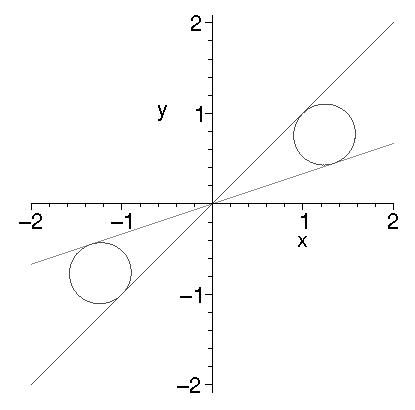
\includegraphics[viewport=0 0 220 220,clip=true]{images/bicircle} \]
 \begin{itemize}
  \item[(a)] Give Maple commands to produce the above picture.
   Include options to ensure that Maple uses the same scale on both
   axes, and that it plots enough points to give a smooth picture of
   $C$. \mrks{7}
  \item[(b)] Find (by hand) the coordinates of the two points where
   $M$ meets $C$. \mrks{5}
 \end{itemize}
\end{problem}
\begin{solution}
 \begin{itemize}
  \item[(a)] 
\begin{verbatim}
with(plots):
f := (x,y) -> (x^2-y^2-1)^2+4*(x*y-1)^2;
display(
 implicitplot(f(x,y)=1,x=-2..2,y=-2..2,grid=[200,200],scaling=constrained), 
 plot([x,x/3],x=-2..2)
);

\end{verbatim}
   (\mk for \verb~display~, \mk for \verb~implicitplot~, \mk for
   ranges, \mk for \verb~grid~ option, \mk for \verb~scaling~ option,
   \mks{2} for \verb~plot~ command)
  \item[(b)] We need to find the points where $y=x/3$ and $f(x,y)=1$.
   We have 
   \begin{align*}
    f(x,x/3) - 1 &= (x^2-x^2/9-1)^2 + 4(x^2/3-1)^2 -1 \\
     &= (8x^2/9-1)^2 + 4(x^2/3-1)^2 - 1\\
     &= 64x^4/81 - 16x^2/9 + 1 + 4x^4/9 - 8x^2/3 + 4 - 1\\
     &= 100x^4/81 -40x^2/9 + 4 \\
     &= 4(5x^2/9-1)^2. \mks{3}
   \end{align*}
   This vanishes when $5x^2/9=1$, so $x=\pm\sqrt{9/5}=\pm 3/\sqrt{5}$.  \mk
   We must also have $y=x/3$, so the intersection points are
   $(-3/\sqrt{5},-1/\sqrt{5})$ and $(3/\sqrt{5},1/\sqrt{5})$. \mk
 \end{itemize}
\end{solution}


\begin{problem}
 \papers{0910}
 Give Maple commands to plot the list of values
 $\frac{10!}{k!(10-k)!}$ for $k=1,2,\dotsc,10$, together with the
 graph of the function $252 e^{-(x-5)^2/5}$ for $0\leq x\leq 10$.
 \mrks{6}
\end{problem}
\begin{solution}
 \begin{verbatim}
with(plots):
display(
 listplot([seq(10!/(k!*(10-k)!),k=1..10)]), 
 plot(252*exp(-(x-5)^2/5),x=0..10)
);
 \end{verbatim}
 (\mk for \verb~display~, \mks{2} for \verb~listplot~, \mk for \verb~seq~,
 \mk for square brackets, \mk for \verb~plot~ command.)
\end{solution}

\begin{problem}
 What would you type to get Maple to draw the curve given
 parametrically by $x=\cos(t)/r$ and $y=\sin(t)/r$, where
 $r=(\cos(t)^8+\sin(t)^8)^{1/8}$ and $t$ runs from $0$ to $2\pi$.
\end{problem}
\begin{solution}
 \begin{verbatim}
  r := (cos(t)^8+sin(t)^8)^(1/8);
  plot([cos(t)/r,sin(t)/r,t=0..2*Pi]);
 \end{verbatim}
\end{solution}

\begin{problem}
 \papers{0708}
 What would you type to get Maple to draw the curve
 $y=\sin(10x)+\sin(11x)$ together with the curve $y=2|\cos(x/2)|$, for
 $-4\pi\leq x\leq 4\pi$? \mrks{4}
\end{problem}
\begin{solution}
 \verb~plot([sin(10*x)+sin(11*x),2*abs(cos(x/2))],x=-4*Pi..4*Pi);~ 
 \mks{4}
\end{solution}

\begin{problem}
 \papers{0506; 0708R}
 \begin{itemize}
  \item[(a)] What would you enter to plot the curve given by
   $x=t-\sin(t)$ and $y=2-\cos(t)$, for $0\leq t\leq 6\pi$?
   You should include an option to make Maple use the same
   scales on the two axes. \mrks{3}
  \item[(b)] What would you enter to plot the curves
   $y=t-\sin(t)$ and $y=2-\cos(t)$ together on the same
   graph, for $0\leq t\leq 6\pi$? \mrks{2}
 \end{itemize}
\end{problem}
\begin{solution}
 \begin{itemize}
  \item[(a)]
   \verb~plot([t-sin(t),2-cos(t),t=0..6*Pi],scaling=constrained);~
   \mks{3}
  \item[(b)]
   \verb~plot([t-sin(t),2-cos(t)],t=0..6*Pi);~
   \mks{2}
 \end{itemize}
\end{solution}


\begin{problem}\label{ex-implicitplot-i}
 \papers{Mock2}
 How would you ask Maple to plot the curve $x^6+y^6=1$ for
 $|x|\leq 3$ and $|y|\leq 3$?  If you found that the picture
 was jagged or inaccurate, how would you improve it? \mrks{4}
\end{problem}
\begin{solution}
 Enter \verb~implicitplot(x^6+y^6=1,x=-3..3,y=-3..3);~ to
 plot the curve \mks{2}.  If it is inaccurate, include the option
 \verb~grid=[100,100]~ \mks{2}. 
\end{solution}

\begin{problem}
 \papers{0405R}
 Consider the function
 \[ f(x,y) = (x-y)^4+(x+y)^4 - x^6 - y^6. \]
 How would you ask Maple to plot the curve $f=0$ for
 $|x|\leq 3$ and $|y|\leq 3$?  If you found that the picture
 was jagged or inaccurate, how would you improve it? \mrks{5}
\end{problem}
\begin{solution}
 Enter \verb~f:=(x,y)->(x-y)^4+(x+y)^4 - x^6 - y^6;~ to
 define the function, then
 \begin{verbatim}
  implicitplot(f(x,y)=0,x=-3..3,y=-3..3);
 \end{verbatim}
 to plot the curve \mks{3}.  (It is perfectly acceptable to
 include the formula in the plot command rather than defining
 a function.)  If it is inaccurate, include the option
 \verb~grid=[100,100]~ \mks{2}. 
\end{solution}

\begin{problem}\label{ex-implicitplot-iii}
 \papers{Mock1}
 How would you ask Maple to plot the lines $y=x$ and $y=-x$
 together with the curve $x^4+y^4=1+9x^2y^2/5$, for
 $-3\leq x,y\leq 3$?  \mrks{6}
\end{problem}
\begin{solution}
\begin{verbatim}
 display(
  plot([x,-x],x=-2..2),
  implicitplot(x^4-9*x^2*y^2/5+y^4=1,
               x=-3..3,y=-3..3,
               grid=[100,100])
 ); 
\end{verbatim}
 \mk for \verb~display()~, \mks{2} for $y=\pm x$, \mks{3} for
 the curve.
\end{solution}

\begin{problem}
 \papers{0506R}
 \begin{itemize}
  \item[(a)] What would you enter to plot the curves
   $y=t^2$ and $y=t(t^2-1)(t^2-2)$ together on the same
   graph?  You should include an option to make Maple show only the
   part of the curve where $-2\leq t\leq 2$ and $-5\leq y\leq 5$. 
   \mrks{4}
  \item[(b)] What would you enter to plot the curve given by
   $x=t^2$ and $y=t(t^2-1)(t^2-2)$, for $-2\leq t\leq 2$?
   You should include an option to make Maple show only the part of
   the curve where $-1\leq x\leq 4$ and $-5\leq y\leq 5$.  \mrks{4}
 \end{itemize}
\end{problem}
\begin{solution}
 \begin{itemize}
  \item[(a)]
   \verb~plot([t^2,t*(t^2-1)*(t^2-2)],t=-2..2,-5..5);~
   \mks{4}
  \item[(b)]
   \verb~plot([t^2,t*(t^2-1)*(t^2-2),t=-2..2],view=[-1..4,-5..5]);~
   \mks{4}
 \end{itemize}
\end{solution}

\begin{problem}\label{ex-implicitplot-ii}
 \papers{0405}
 How would you ask Maple to plot the curve
 $(x+\sin(2\pi x))^2+y^2=4$, with the same scale on the $x$
 and $y$ axes?  You should decide for yourself what is an
 appropriate range for the axes.  You should also include an
 option telling Maple to plot extra points, so as to give a
 picture of reasonable quality.  \mrks{5}
\end{problem}
\begin{solution}
\begin{verbatim}
 plots[implicitplot](
  (x+sin(2*Pi*x))^2+y^2=4,
  x=-3..3,y=-3..3,
  scaling=constrained,
  grid=[200,200]
 );
\end{verbatim}
 \mk for \verb~implicitplot~, \mk for
 \verb~x+sin(2*Pi*x))^2+y^2=4~, \mk for ranges, \mk
 for \verb~scaling=constrained~, \mk for
 \verb~grid=[..,..]~.  (Any grid size is acceptable.)
\end{solution}

\begin{problem}\label{ex-ellipse}
 \papers{Mock2}
 Consider the curve $C$ given parametrically by the
 equations $x=2\cos(t)+3\sin(t)$ and $y=2\cos(t)-3\sin(t)$:
 \[ \includegraphics[viewport=0 0 200 130,clip=true]{images/ellipse} \]
 \begin{itemize}
  \item[(a)] How would you generate the above picture?  (You
   need not include commands to mark or label the points $P$
   and $Q$.) \mrks{3}
  \item[(b)] How would you ask Maple to find the coordinates
   of the point $P$, where the curve crosses the $y$-axis?
   \mrks{3}
  \item[(c)] How would you ask Maple to find the coordinates
   of the point $Q$ (the highest point on the curve)?
   \mrks{3}
 \end{itemize}
\end{problem}
\begin{solution}
 \begin{itemize}
  \item[(a)] 
\begin{verbatim}
 x := 2*cos(t)+3*sin(t);
 y := 2*cos(t)-3*sin(t);
 plot([x,y,t=0..2*Pi]);
\end{verbatim}
   \mks{3}
  \item[(b)]
   \verb~sol := solve(x=0,{t}); subs(sol[1],[x,y]);~  
   \hspace{3em} \mks{3}
  \item[(c)] \verb~sol := solve(diff(y,t)=0,{t}); subs(sol[1],[x,y]);~
   \hspace{3em} \mks{3}
 \end{itemize}
\end{solution}

\begin{problem}
 \papers{0506; 0708R}
 The following picture shows the curve $x^4-3x^2+1=-y^2$,
 together with the lines $y=x$ and $y=-x$.
 \[ \includegraphics[viewport=10 10 600 450,clip=true,scale=0.4]{images/jacobi} \]
 \begin{itemize}
  \item[(a)] How would you generate the above picture?
   (You should include an option to ensure that Maple plots
   enough points to give a smooth picture.) \mrks{6}
  \item[(b)] Let $P$ and $Q$ be the points where the curve
   meets the line $y=-x$.  What would you enter in Maple to
   find the coordinates of $P$ and $Q$? \mrks{2}
  \item[(c)] Find the coordinates of $P$ and $Q$ by hand.
   \mrks{4}
 \end{itemize}
\end{problem}
\begin{solution}
 \begin{itemize}
  \item[(a)]
\begin{verbatim}
 with(plots):
 display(
  implicitplot(x^4-3*x^2+1=-y^2,x=-2..2,y=-2..2,grid=[200,200]),
  plot(x,x=-2..2),
  plot(-x,x=-2..2)
 );
\end{verbatim}
  \mk for \verb~display()~, \mks{3} for the curve, \mks{2}
  for the lines.  No penalty for omitting \verb~with(plots)~.
 \item[(b)] \verb~solve(x^4-3*x^2+1=-(-x)^2,{x});~. \mks{2}
 \item[(c)] We have to solve $x^4-3x^2+1=-x^2$ \mk, or equivalently
  $x^4-2x^2+1=0$, or equivalently $(x^2-1)^2=0$ \mk.  The
  solutions are $x=\pm 1$ \mk, so the intersection points are
  $(1,-1)$ and $(-1,1)$ \mk.
 \end{itemize}
\end{solution}


\begin{problem}
 \papers{0405R}
 Consider the following picture:
 \[ \includegraphics[viewport=0 0 200 130,clip=true]{images/doodle} \]
 It shows the curve $C$ given parametrically by the
 equations
 \begin{eqnarray*}
  x &=& 10\cos(t) + \sin(11t) \\
  y &=& 10\sin(t) + \cos(9t),
 \end{eqnarray*}
 together with a semicircle of radius $12$ in the upper half
 plane, and a semicircle of radius $8$ in the lower half
 plane.  What Maple command would you use to generate this
 picture? \mrks{7}
\end{problem}
\begin{solution}
 \begin{verbatim}
  plots[display](
   plot([10*cos(t)+sin(11*t),10*sin(t)+cos(9*t),t=0..2*Pi]),
   plot([12*cos(t),12*sin(t),t=0..Pi]),
   plot([8*cos(t),8*sin(t),t=Pi..2*Pi])
  );
 \end{verbatim}
 \mk for \verb~display~, then \mks{3} for the curve, then
 \mks{2} for the first semicircle, and \mk for the other
 one. 
\end{solution}

\begin{problem}
 \papers{0506R}
 The following picture shows the curve $C$ with equation
 $x=\sin(2t)\sin(t)$ and $y=\sin(2t)\cos(t)$, together with the circle
 of radius one centred at the origin.
 \[ \includegraphics[scale=0.3]{images/clover.jpg} \]
% \[ \includegraphics[scale=0.3]{images/clover.pdf} \]
 \begin{itemize}
  \item[(a)] How would you generate the above picture? \mrks{6}
  \item[(b)] What are the coordinates of the four points at which $C$
   meets the circle?  (You may guess the answer, but you should then
   give an argument to show that your guess is correct.) \mrks{4}
 \end{itemize}
\end{problem}
\begin{solution}
 \begin{itemize}
  \item[(a)]
\begin{verbatim}
 with(plots):
 display(
  plot([sin(2*t)*sin(t),sin(2*t)*cos(t),t=0..2*Pi]),
  plot([sin(t),cos(t),t=0..2*Pi])
 );
\end{verbatim}
  \mk for \verb~display()~, \mks{3} for the curve, \mks{2}
  for the circle.  No penalty for omitting \verb~with(plots)~.
 \item[(b)] The intersection points are
  $(x,y)=(\pm 1,\pm 1)/\sqrt{2}$ \mks{2}.  Indeed, these points are
  certainly on the unit circle \mk, and $C$ passes through them at
  $t=\pi/4$, $t=3\pi/4$, $t=5\pi/4$ and $t=7\pi/4$ \mk. 
 \end{itemize}
\end{solution}

\begin{problem}
 \papers{0708}
 The picture below shows the curve $C$ with equation $y^2=x^3-x$, the
 curve $C'$ given parametrically by $x=t^2$ and $y=t^3$ with
 $-\sqrt{2}\leq t\leq\sqrt{2}$, and the line $L$ of slope $1-\sqrt{2}$
 passing through the point $(1,0)$.
 \[ \includegraphics[viewport=100 90 700 500,clip=true,scale=0.4]{images/ell} \]
 \begin{itemize}
  \item[(a)] What is the equation of $L$? \mrks{2}
  \item[(b)] How would you generate the above picture?
   (You should include an option to ensure that Maple plots
   enough points to give a smooth picture. You may assume that the
   \verb~plots~ package has already been loaded.) \mrks{9}
  \item[(c)] The line $L$ meets $C$ at $(1,0)$ and also at another
   point $P$.  How would you ask Maple to find the coordinates of $P$?
   \mrks{3}
 \end{itemize}
\end{problem}
\begin{solution}
 \begin{itemize}
  \item[(a)] The equation of $L$ is $y=(1-\sqrt{2})(x-1)$. \mks{2}
  \item[(b)] 
\begin{verbatim}
display(
  implicitplot(y^2=x^3-x,x=-2..2,y=-2..2,grid=[200,200]),
  plot([t^2,t^3,t=-sqrt(2)..sqrt(2)]),
  plot((1-sqrt(2))*(x-1),x=-1..2)
);
\end{verbatim}
  \mk for \verb~display~, \mks{3} for the implicit plot, \mks{3} for
  the parametric plot, \mks{2} for the line.
 \item[(c)] \verb~solve({y^2=x^3-x,y=(1-sqrt(2))*(x-1)},{x,y});~
  \mks{3} (\verb~fsolve~ would also be acceptable.)
 \end{itemize}
\end{solution}

\begin{problem}\label{ex-nodal}
 \papers{0405}
 The picture below shows the unit circle, together with the
 curve $C$ given by $x=1-t^2$ and $y=t-t^3$, for
 $-3/2\leq t\leq 3/2$.  
 \[ \includegraphics[viewport=0 0 200 200,clip=true]{images/nodal} \]
 \begin{itemize}
  \item[(a)] How would you generate the above picture?  (You
   need not include commands to mark or label the points $P$,
   $Q$ and $R$.) \mrks{5}
  \item[(b)] How would you ask Maple to find the values of
   $t$ at the points $P$, $Q$ and $R$ where the curve meets
   the circle?  (Do not worry about the possibility of
   spurious complex roots.)  \mrks{3}
  \item[(c)] Given that $t=\sqrt{2+2\sqrt{5}}/2$ at $Q$, how
   would you ask Maple to find the coordinates of $Q$?
   \mrks{2}
 \end{itemize} 
\end{problem}
\begin{solution}
 \begin{itemize}
  \item[(a)] 
\begin{verbatim}
 plots[display](
  plot([cos(t),sin(t),t=0..2*Pi]),
  plot([1-t^2,t-t^3,t=-3/2..3/2]),
  scaling=constrained
 );
\end{verbatim}
   \mk for \verb~display()~, \mks{2} for the circle, \mks{2}
   for the curve.  No penalty for omitting \verb~plots[...]~
   or \verb~scaling=constrained~.  
  \item[(b)] 
\begin{verbatim}
 x := 1-t^2;
 y := t-t^3;
 sols := solve(x^2+y^2=1,{t});
\end{verbatim}
  (This will find two complex values of $t$ as well, but I
  will ignore that.)
  \mks{3}
  \item[(c)] \verb~subs(t=sqrt(2+2*sqrt(5))/2,[x,y]);~  \mks{2}
 \end{itemize}
\end{solution}

\begin{problem}\label{ex-reveng}
 \papers{Mock1}
 Here is a graph of the function $y=1/(x^3-x)$:
 \[ \includegraphics[viewport=0 0 200 130,clip=true]{images/reveng} \]
 What Maple command would you use to generate this plot?
 Your command should reproduce the following features:
 \begin{itemize}
  \item The horizontal and vertical ranges are as shown.
  \item The distance from $0$ to $2$ is the same on the two
   axes.
  \item There are no vertical lines at the points of
   discontinuity. 
  \item The axes appear on the outside of the plot, rather
   than passing through the origin.
 \end{itemize}
 \mrks{4}
\end{problem}
\begin{solution}
\begin{verbatim}
 plot(1/(x^3-x),x=-4..4,-6..6,
      axes=boxed,
      scaling=constrained,
      discont=true):
\end{verbatim}
 \mks{4}
\end{solution}

\begin{problem}\label{ex-tricorn}
 \papers{0809}

 Consider the curve $C$ given parametrically by the
 equations $x=2\sin(t)+\sin(2t)$ and $y=-2\cos(t)+\cos(2t)$.
 The picture below shows $C$ together with two circles centred at the
 origin. 
 \[ 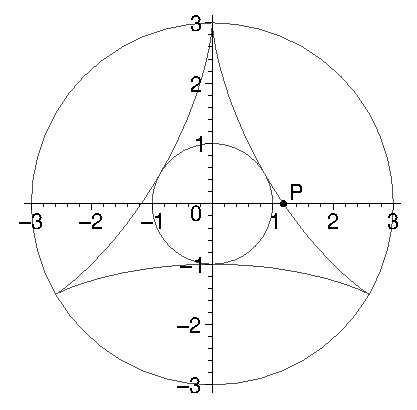
\includegraphics[viewport=0 0 220 220,clip=true]{images/tricorn} \]
 \begin{itemize}
  \item[(a)] How would you generate the above picture?  (You need not
   include commands to mark the point $P$.) \mrks{5}
  \item[(b)] Write down the addition formula for $\cos(a+b)$.\mrks{1}
  \item[(c)] Show that $x^2+y^2=5-4\cos(3t)$, and
   thus that $1\leq x^2+y^2\leq 9$. \mrks{5}
  \item[(d)] Explain how~(b) relates to the geometry of the
   picture. \mrks{1} 
%  \item[(e)] Give a formula for $dy/dx$ in terms of $t$. \mrks{3}
%  \item[(f)] Prove that $(x^2+y^2+12y+9)^2=4(2y+3)^3$.
  \item[(e)] There is a point $P$ close to $t=2$ where $y=0$.  What
   would you enter in Maple to find the approximate values of $t$ and
   $x$ at $P$, to 100 decimal places? \mrks{5}
 \end{itemize}
\end{problem}
\begin{solution}
 \begin{itemize}
  \item[(a)]
   \begin{verbatim}
x := 2*sin(t)+sin(2*t);
y := -2*cos(t)+cos(2*t);
plots[display](
 plot([x,y,t=0..2*Pi]),
 plot([cos(t),sin(t),t=0..2*Pi]),
 plot([3*cos(t),3*sin(t),t=0..2*Pi])
);
   \end{verbatim}
   \mks{5}
  \item[(b)] $\cos(a+b)=\cos(a)\cos(b)-\sin(a)\sin(b)$. \mk
  \item[(c)] We have
   \begin{align*}
    x^2+y^2
     &= 4\sin(t)^2+4\sin(t)\sin(2t)+\sin(2t)^2 +
        4\cos(t)^2-4\cos(t)\cos(2t)+\cos(2t)^2 \mk \\
     &= 5-4(\cos(t)\cos(2t)-\sin(t)\sin(2t)) \mk \\
     &= 5-4\cos(3t). \mk
   \end{align*}
   (Here the last step used part~(b).)  Moreover, $\cos(3t)$ runs
   between $-1$ and $+1$, so $5-4\cos(3t)$ runs between $5-4=1$ and
   $5+4=9$.  Thus $1\leq x^2+y^2\leq 9$. \mks{2}
  \item[(d)] Geometrically this means that the curve $C$ lies between
   the circles of radius $\sqrt{1}=1$ and $\sqrt{9}=3$ centred at the
   origin, which is also clear from the picture. \mk
%  \item[(e)] We have
%   \[ \frac{dy}{dx} = 
%      \frac{dy/dt}{dx/dt} \mk = 
%      \frac{2\sin(t)-2\sin(2t)}{2\cos(t)+2\cos(2t)} =
%      \frac{\sin(t)-\sin(2t)}{\cos(t)+\cos(2t)} \mks{2}.
%   \]
%   (This can in fact be simplified further to $-\sin(t)/(1+\cos(t))$,
%   but that is not required for full credit.)
  \item[(e)]
   \begin{verbatim}
Digits := 100;
t0 := fsolve(y=0, t=2);
x0 := evalf(subs(t=t0,x));
   \end{verbatim}
  (\mk, \mks{2}, \mks{2})
 \end{itemize}
\end{solution}


\subsection{Numerical evaluation}

\begin{problem}\label{ex-evalf-i}
 \papers{0405}
 What would you enter in Maple to calculate $\log_{2}(\pi)$
 to $50$ decimal places?  \mrks{2}
\end{problem}
\begin{solution}
 \verb~evalf[50](log[2](Pi));~ \mks{2}
 (1/2 mark each for \verb~evalf~, \verb~[50]~,
 \verb~log[2]~, \verb~Pi~; halves rounded down.  It is
 acceptable (in fact, preferable) to use \verb~Digits:=50;~
 rather than giving 50 as an index to \verb~evalf~.)
\end{solution}

\begin{problem}\label{ex-evalf-iii}
 \papers{Mock2}
 What would you enter in Maple to calculate $\ln(\ln(\ln(\pi)))$
 to $40$ decimal places? \mrks{2}
\end{problem}
\begin{solution}
 \verb~evalf[40](ln(ln(ln(Pi))));~ \mks{2}
\end{solution}

\begin{problem}\label{ex-evalf-ii}
 \papers{Mock1}
 What would you enter in Maple to calculate $\sin(2^{3^6-3})$
 to $1000$ decimal places?  \mrks{2}
\end{problem}
\begin{solution}
 \verb~evalf[1000](sin(2^(3^6-3)));~ \hspace{2em}\mks{2}
\end{solution}



\subsection{Fixing errors}

\begin{problem}
 \papers{0910}
 The following table shows some Maple commands, together
 with the output that the user expected to get.  In each
 case, the command has one or more errors, so the output
 would not be as expected.  Give a corrected version of each
 command.   \mrks{9}
 \[ \renewcommand{\arraystretch}{2}
    \begin{array}{|c|l|l|}
     \hline
      & \text{Input} & \text{Expected output} \\ \hline
      \text{(a)} &
      \verb~digits=15;eval(pi);~ &
      3.14159265358979 \\ \hline
      \text{(b)} &
      \verb~solve(ax+b=0);~ &
      \{x=-b/a\} \\ \hline
      \text{(c)} &
      \verb~dif(t^3);~ &
      3t^2 \\ \hline
    \end{array}
 \]
\end{problem}
\begin{solution}
 \begin{itemize}
  \item[(a)] \verb~Digits:=15;evalf(Pi);~      \hspace{2em}\mks{4}
  \item[(b)] \verb~solve(a*x+b=0,{x});~        \hspace{2em}\mks{3}
  \item[(c)] \verb~diff(t^3,t);~                \hspace{2em}\mks{2}
 \end{itemize}
\end{solution}

\begin{problem}\label{ex-error-ii}
 \papers{Mock2; 0708R}
 The following table shows some Maple commands, together
 with the output that the user expected to get.  In each
 case, the command has one or more errors, so the output
 would not be as expected.  Give a corrected version of each
 command.  \mrks{6}
 \[ \renewcommand{\arraystretch}{2}
    \begin{array}{|c|l|l|}
     \hline
      & \text{Input} & \text{Expected output} \\ \hline
      \text{(a)} &
      \verb~simplify((xy+y)/(x+1));~ &
      y \\ \hline
      \text{(b)} &
      \verb~Expand(((a+b)*-c);~ &
      -ac-bc \\ \hline
      \text{(c)} &
      \verb~diff(x^2);~ &
      2x \\ \hline
      \text{(d)} &
      \verb~f(x)=x^2; f(3);~ &
      9 \\ \hline
    \end{array}
 \]
\end{problem}
\begin{solution}
 \begin{itemize}
  \item[(a)] \verb~simplify((x*y+y)/(x+1));~ \hspace{2em}\mks{1}
  \item[(b)] \verb~expand((a+b)*(-c));~ \hspace{2em}\mks{2}
  \item[(c)] \verb~diff(x^2,x);~ \hspace{2em}\mks{1}
  \item[(d)] \verb~f := (x)->x^2; f(3);~ \hspace{2em}\mks{2}
 \end{itemize}
\end{solution}

\begin{problem}\label{ex-error-iii}
 \papers{0405; 0809}
 The following table shows some Maple commands, together
 with the output that the user expected to get.  In each
 case, the command has one or more errors, so the output
 would not be as expected.  Give a corrected version of each
 command.   \mrks{8}
 \[ \renewcommand{\arraystretch}{2}
    \begin{array}{|c|l|l|}
     \hline
      & \text{Input} & \text{Expected output} \\ \hline
      \text{(a)} &
      \verb~solve(x+y:=2,x-y:=0,x,y);~ &
      \{x=1,y=1\} \\ \hline
      \text{(b)} &
      \verb~simplify(Sqrt(a^-8));~ &
      a^{-4} \\ \hline
      \text{(c)} &
      \verb~solve(cos(5*x)=0,x);~ &
      \{x = 0.3141592654\} \\ \hline
      \text{(d)} &
      \verb~simplify([x^2-y^2]/[x+y]);~ &
      x-y \\ \hline
    \end{array}
 \]
\end{problem}
\begin{solution}
 \begin{itemize}
  \item[(a)] \verb~solve({x+y=2,x-y=0},{x,y});~      \hspace{2em}\mks{2}
  \item[(b)] \verb~simplify(sqrt(a^(-8)),symbolic);~ \hspace{2em}\mks{3}
  \item[(c)] \verb~fsolve(cos(5*x)=0,{x});~          \hspace{2em}\mks{2}
  \item[(d)] \verb~simplify((x^2-y^2)/(x+y));~       \hspace{2em}\mk
 \end{itemize}
\end{solution}

\begin{problem}
 \papers{0506R}
 The following table shows some Maple commands, together
 with the output that the user expected to get.  In each
 case, the command has one or more errors, so the output
 would not be as expected.  Give a corrected version of each
 command.   \mrks{10}
 \[ \renewcommand{\arraystretch}{2}
    \begin{array}{|c|l|l|}
     \hline
      & \mbox{Input} & \mbox{Expected output} \\ \hline
      \mbox{(a)} &
      \verb~Simplify(a^2-b^2/a-b);~ &
      a+b \\ \hline
      \mbox{(b)} &
      \verb~solve(x+3=pi);~ &
      \{x=0.1415926540\} \\ \hline
      \mbox{(c)} &
      \verb~xy^-3/xy;~ &
      1/y^4 \\ \hline
      \mbox{(d)} &
      \verb~[seq(n^2,1..5)];~ &
      [1,4,9,16,25] \\ \hline
    \end{array}
 \]
\end{problem}
\begin{solution}
 \begin{itemize}
  \item[(a)] \verb~simplify((a^2-b^2)/(a-b));~         \hspace{2em}\mks{2}
  \item[(b)] \verb~fsolve(x+3=Pi,{x});~               \hspace{2em}\mks{3}
  \item[(c)] \verb~x*y^(-3)/(x*y);~                 \hspace{2em}\mks{4}
  \item[(d)] \verb~[seq(n^2,n=1..5)];~         \hspace{2em}\mks{1}
 \end{itemize}
\end{solution}

\begin{problem}\label{ex-error-i}
 \papers{Mock1}
 The following table shows some Maple commands, together
 with the output that the user expected to get.  In each
 case, the command has one or more errors, so the output
 would not be as expected.  Give a corrected version of each
 command.  \mrks{7}
 \[ \renewcommand{\arraystretch}{2}
    \begin{array}{|c|l|l|}
     \hline
      & \text{Input} & \text{Expected output} \\ \hline
      \text{(a)} &
      \verb~Sin(2 pi);~ &
      0 \\ \hline
      \text{(b)} &
      \verb~simplify((x^2-y^2)(X-Y)^-1);~ &
      x+y \\ \hline
      \text{(c)} &
      \verb~x := 1; unassign(x); expand((1+x)^2);~ &
      1 + 2x + x^2 \\ \hline
      \text{(d)} &
      \verb~ln(e^2(x+y));~ &
      2(x+y) \\ \hline
    \end{array}
 \]
\end{problem}
\begin{solution}
 \begin{itemize}
  \item[(a)] \verb~sin(2*Pi);~  \hspace{2em}\mks{2}
  \item[(b)] \verb~simplify((x^2-y^2)*(x-y)^(-1));~ \hspace{2em}\mks{2}
  \item[(c)] \verb~x := 1; unassign('x'); expand((1+x)^2);~ \hspace{2em}\mks{1}
  \item[(d)] \verb~ln(exp(2*(x+y)));~ \hspace{2em}\mks{2}
 \end{itemize}
 (For part~(d), you really need
 \verb~simplify(ln(exp(2*(x+y))),symbolic);~ to get $2(x+y)$
 as the answer, but the answer given above would be accepted
 as correct.)
\end{solution}

\begin{problem}
 \papers{0405R}
 The following table shows some Maple commands, together
 with the output that the user expected to get.  In each
 case, the command has one or more errors, so the output
 would not be as expected.  Give a corrected version of each
 command.  \mrks{7}
 \[ \renewcommand{\arraystretch}{2}
    \begin{array}{|c|l|l|}
     \hline
      & \mbox{Input} & \mbox{Expected output} \\ \hline
      \mbox{(a)} &
      \verb~simplify((xy+y)/(x+1));~ &
      y \\ \hline
      \mbox{(b)} &
      \verb~Expand((a+b)(a-b)*-1);~ &
      b^2-a^2 \\ \hline
      \mbox{(c)} &
      \verb~diff(x^4);~ &
      4x^3 \\ \hline
      \mbox{(d)} &
      \verb~e^2log(x);~ &
      x^2 \\ \hline
    \end{array}
 \]
\end{problem}
\begin{solution} 
 \begin{itemize}
  \item[(a)] \verb~simplify((x*y+y)/(x+1));~ \hspace{2em}\mks{1}
  \item[(b)] \verb~expand((a+b)*(a-b)*(-1));~ \hspace{2em}\mks{3}
  \item[(c)] \verb~diff(x^4,x);~ \hspace{2em}\mks{1}
  \item[(d)] \verb~exp(2*log(x));~ \hspace{2em}\mks{2}
 \end{itemize}
\end{solution}

\begin{problem}
 \papers{0506}
 The following table shows some Maple commands, together
 with the output that the user expected to get.  In each
 case, the command has one or more errors, so the output
 would not be as expected.  Give a corrected version of each
 command.   \mrks{10}
 \[ \renewcommand{\arraystretch}{2}
    \begin{array}{|c|l|l|}
     \hline
      & \mbox{Input} & \mbox{Expected output} \\ \hline
      \mbox{(a)} &
      \verb~Expand((a+b)(a-b));~ &
      a^2-b^2 \\ \hline
      \mbox{(b)} &
      \verb~pi^-2;~ &
      0.1013211836 \\ \hline
      \mbox{(c)} &
      \verb~solve(tan(x)+1=a);~ &
      \{x = \arctan(a-1)\} \\ \hline
      \mbox{(d)} &
      \verb~seq(ln(10..13));~ &
      [\ln(10),\ln(11),\ln(12),\ln(13)] \\ \hline
    \end{array}
 \]
\end{problem}
\begin{solution}
 \begin{itemize}
  \item[(a)] \verb~expand((a+b)*(a-b));~         \hspace{2em}\mks{2}
  \item[(b)] \verb~evalf(Pi^(-2));~               \hspace{2em}\mks{3}
  \item[(c)] \verb~solve(tan(x)+1=a,{x});~          \hspace{2em}\mks{2}
  \item[(d)] \verb~[seq(ln(n),n=10..13)];~         \hspace{2em}\mks{3}
 \end{itemize}
\end{solution}


\begin{problem}
 \papers{0708}
 The following table shows some Maple commands, together
 with the output that the user expected to get.  In each
 case, the command has one or more errors, so the output
 would not be as expected.  Give a corrected version of each
 command.   \mrks{9}
 \[ \renewcommand{\arraystretch}{2}
    \begin{array}{|c|l|l|}
     \hline
      & \mbox{Input} & \mbox{Expected output} \\ \hline
      \mbox{(a)} &
      \verb~Log(e^a);~ &
      a \\ \hline
      \mbox{(b)} &
      \verb~y=1/(1+t); solve(y:=3/4,t);~ &
      0.3333333333 \\ \hline
      \mbox{(c)} &
      \verb~factor([t^4-1]/[(t-1)(t+1)]);~ &
      t^2+1 \\ \hline
      \mbox{(d)} &
      \verb~seq(x^n,5..7);~ &
      [x^5,x^6,x^7] \\ \hline
    \end{array}
 \]
\end{problem}
\begin{solution}
 \begin{itemize}
  \item[(a)] \verb~simplify(log(exp(a)),symbolic);~
   \hspace{2em}\mks{2}\\
   (No penalty for omitting \verb~simplify(...,symbolic)~)
  \item[(b)] \verb~y:=1/(1+t): fsolve(y=3/4,t);~ \hspace{2em}\mks{3}\\
   (No penalty for semicolon instead of colon)
  \item[(c)] \verb~factor((t^4-1)/((t-1)*(t+1)));~ \hspace{2em}\mks{2}\\
   (\verb~simplify()~ will do instead of \verb~factor()~)
  \item[(d)] \verb~[seq(x^n,n=5..7)];~         \hspace{2em}\mks{2}
 \end{itemize}
\end{solution}

\subsection{Conversion and simplification}

\begin{problem}
 \papers{0506R; 0809}
 Suppose that the following definitions have been made:
 \begin{eqnarray*}
  P &=& 1+x+x^2+O(x^3) \\
  Q &=& 6t^3+7t^2-1 \\
  R &=& (1+3X+3X^2+X^3)^{1/3} \\
  S &=& a^4b + ab^2 + ab^3 + a^4b^4
 \end{eqnarray*}
 \begin{itemize}
  \item[(a)] What would you enter to convert $P$ to the form
   $1+x+x^2$? 
  \item[(b)] What would you enter to convert $Q$ to the form
   $(3t-1)(2t+1)(t+1)$?
  \item[(c)] What would you enter to convert $R$ to the form
   $1+X$?
  \item[(d)] What would you enter to convert $S$ to the form
   $(b+b^4)a^4+(b^2+b^3)a$?
 \end{itemize}
 \mrks{4}
\end{problem}
\begin{solution}
 \begin{itemize}
  \item[(a)] \verb~convert(P,polynom);~  \mk
  \item[(b)] \verb~factor(Q);~ \mk
  \item[(c)] \verb~simplify(R,symbolic);~ \mk
  \item[(d)] \verb~collect(S,a);~ \mk
 \end{itemize}
\end{solution}

\begin{problem}
 \papers{0506}
 Suppose that the following definitions have been made:
 \begin{eqnarray*}
  P &=& 1+x+x^2+x^3+x^4+x^5+x^6+x^7 \\
  Q &=& t+t^4+t^9 + O(t^{16}) \\
  R &=& uv + uv^2 +u^2v^2 + u^2v^3 + u^3v^3 + u^3v^4 \\
  S &=& \sqrt{1 + 2u^4 + u^8}
 \end{eqnarray*}
 \begin{itemize}
  \item[(a)] What would you enter to convert $P$ to the form
   $(x+1)(x^2+1)(x^4+1)$? 
  \item[(b)] What would you enter to convert $Q$ to the form
   $t+t^4+t^9$?
  \item[(c)] What would you enter to convert $R$ to the form
   $(v^3+v^4)u^3+(v^2+v^3)u^2+(v+v^2)u$?
  \item[(d)] What would you enter to convert $S$ to the form
   $1+u^4$?
 \end{itemize}
 \mrks{4}
\end{problem}
\begin{solution}
 \begin{itemize}
  \item[(a)] \verb~factor(P);~  \mk
  \item[(b)] \verb~convert(Q,polynom);~ \mk
  \item[(c)] \verb~collect(R,u);~ \mk
  \item[(d)] \verb~simplify(S,symbolic);~ \mk
 \end{itemize}
\end{solution}

\begin{problem}\label{ex-algebra-i}
 \papers{0405}
 The following expressions are all mathematically equivalent:
 \begin{itemize}
  \item[(a)] $u^3q^3-u^3q^2-u^2q^2+u^2q-uq^2+uq+q-1$
  \item[(b)] $(q-1)(u q-1)(u^2 q-1)$
  \item[(c)] $(q^3-q^2)u^3+(-q^2+q)u^2+(-q^2+q)u+q-1$
  \item[(d)] $u^3q^3+(-u^3-u^2-u)q^2+(u^2+u+1)q-1$
 \end{itemize}
 Suppose that \verb~A~ has been set equal to
 expression~(a).  What would you enter in Maple to convert
 this to forms~(b), (c) and~(d)?  (Do not worry about the
 precise ordering of terms.)  \mrks{3}
\end{problem}
\begin{solution}
 \begin{itemize}
  \item[(b)] \verb~factor(A);~    \hspace{2em}\mk
  \item[(c)] \verb~collect(A,u);~ \hspace{2em}\mk
  \item[(d)] \verb~collect(A,q);~ \hspace{2em}\mk
 \end{itemize}
\end{solution}

\begin{problem}\label{ex-algebra-ii}
 \papers{Mock1}
 The following expressions are all mathematically equivalent:
 \begin{itemize}
  \item[(a)] $y^2x^2+yx^3+x^4+yx+1/yx^3+x^2+1/yx+1/y^2x^2+1$
  \item[(b)] $1+x(y+1/y)+x^2(y^2+1+1/(y^2))+(y+1/y)x^3+x^4$
  \item[(c)] $(y^2x^2+1+yx)(y^2+yx+x^2)/y^2$
  \item[(d)] $x^2y^2+(x+x^3)y+x^4+x^2+1+(x+x^3)y^{-1}+x^2y^{-2}$
 \end{itemize}
 Suppose that \verb~A~ has been set equal to
 expression~(a).  What would you enter in Maple to convert
 this to forms~(b), (c) and~(d)?  (Do not worry about the
 precise ordering of terms.)  \mrks{3}
\end{problem}
\begin{solution}
 \begin{itemize}
  \item[(b)] \verb~collect(A,x);~  \hspace{2em}\mk
  \item[(c)] \verb~factor(A);~     \hspace{2em}\mk
  \item[(d)] \verb~collect(A,y);~  \hspace{2em}\mk
 \end{itemize}
\end{solution}

\begin{problem}\label{ex-algebra-iii}
 \papers{Mock2}
 Suppose that Maple variables $a$, $b$ and $c$ have been
 given the following values:
 \begin{align*}
  a &= 1+x+xy+xy^2+x^2y+x^2y^2+x^2y^3+x^3y^3 \\
  b &= x^3y^3 + (y^3+y^2+y)x^2 + (y^2+y+1)x + 1 \\
  c &= (1+x)(1+xy)(1+xy^2).
 \end{align*}
 All three expressions are mathematically equivalent.
 \begin{itemize}
  \item[(i)] What Maple command would you use to convert
   form $a$ to form $b$? \mrks{1}
  \item[(ii)] What Maple command would you use to convert
   form $b$ to form $a$? \mrks{1}
  \item[(iii)] What Maple command would you use to convert
   form $a$ to form $c$? \mrks{1}
 \end{itemize}
\end{problem}
\begin{solution}
 \begin{itemize}
  \item[(i)] \verb~collect(a,x);~  \hspace{2em}\mks{1}
  \item[(ii)] \verb~expand(b);~    \hspace{2em}\mks{1}
  \item[(iii)] \verb~factor(a);~   \hspace{2em}\mks{1}
 \end{itemize}
\end{solution}

\begin{problem}\label{ex-root-power-i}
 \papers{Mock1}
 What Maple command would you use to convert $(x^4)^{1/4}$
 to $x$?  Explain why this conversion is not always valid.
 \mrks{3}
\end{problem}
\begin{solution}
 The relevant command is
 \verb~simplify((x^4)^(1/4),symbolic);~  \mk.  The resulting
 simplification is not always valid because when $x$ is
 negative we have $(x^4)^{1/4}=|x|\neq x$  \mks{2}.
\end{solution}


\begin{problem}\label{ex-root-power-ii}
 \papers{0405}
 What Maple command would you use to convert
 $\sqrt{p^2+2pq+q^2}$ to $p+q$?  Explain why this conversion
 is not always valid.  \mrks{3}
\end{problem}
\begin{solution}
 The relevant command is
 \verb~simplify(sqrt(p^2+2*p*q+q^2),symbolic);~ \hspace{1em}
 \mk.  The resulting simplification is not always valid
 because when $p+q$ is negative we have
 $\sqrt{p^2+2pq+q^2}=|p+q|\neq p+q$ \mks{2}.
\end{solution}

\begin{problem}
 \papers{0405R}
 What Maple command would you use to convert
 $\arcsin(\sin(x))$ to $x$?  Give an example of a value of
 $x$ for which this simplification is not valid.  \mrks{4}
\end{problem}
\begin{solution}
 The relevant command is
 \verb~simplify(arcsin(sin(x)),symbolic);~.  \mk The resulting
 simplification is not valid when $x=2\pi$ (for example): we
 have $\sin(2\pi)=0$ and so 
 \[ \arcsin(\sin(2\pi))=\arcsin(0)=0\neq 2\pi.   \mks{3} \] 
\end{solution}

\begin{problem}\label{ex-simp-symb}
 \papers{Mock2}
 What Maple command would you use to convert
 $\arccos(\cos(x))$ to $x$?  Give an example of $x$ for
 which this simplification is not valid.  \mrks{4}
\end{problem}
\begin{solution}
 The relevant command is
 \verb~simplify(arccos(cos(x)),symbolic);~.  \mk The resulting
 simplification is not valid when $x=2\pi$ (for example): we
 have $\cos(2\pi)=1$ and so 
 \[ \arccos(\cos(2\pi))=\arccos(1)=0\neq 2\pi.   \mks{3} \] 
\end{solution}

\begin{problem}
 \papers{0405R}
 \begin{itemize}
  \item[(i)] What Maple command would you use to convert
   the expression $x^4-y^4$ to the form $(x-y)(x+y)(x^2+y^2)$? \mrks{1}
  \item[(ii)] What Maple command would you use to convert
   the expression $a^2+ab+a^3+a^2b+ab^2$ to the form 
   $a^3+(1+b)a^2+(b+b^2)a$? \mrks{1}
  \item[(iii)] What Maple command would you use to convert
   the expression $(x+1/x)^4$ to the form $x^4+4x^2+6+4x^{-2}+x^{-4}$? \mrks{1}
 \end{itemize}
\end{problem}
\begin{solution}
 \begin{itemize}
  \item[(i)] \verb~factor(x^4-y^4);~  \hspace{2em}\mks{1}
  \item[(ii)] \verb~collect(a^2+a*b+a^3+a^2*b+a*b^2,a);~
    \hspace{2em}\mks{1}
  \item[(iii)] \verb~expand((x+1/x)^4);~   \hspace{2em}\mks{1}
 \end{itemize}
\end{solution}




\subsection{Sequences}

\begin{problem}\label{ex-seq-i}
 \papers{0405}
 What would you enter in Maple to generate the sequence
 $1,x^2,x^4,x^6,\ldots,x^{100}$?  \mrks{2}
\end{problem}
\begin{solution}
 \verb~seq(x^(2*k),k=0..50);~ \hspace{2em}\mks{2}
\end{solution}

\begin{problem}\label{ex-seq-iii}
 \papers{Mock2; 0405R}
 What would you enter in Maple to generate the sequence
 $dy/dx,d^2y/dx^2,\dotsc,d^{10}y/dx^{10}$?  \mrks{3}
\end{problem}
\begin{solution}
 \verb~seq(diff(y,x$k),k=1..10);~  \hspace{3em} \mks{3}
\end{solution}

\begin{problem}\label{ex-seq-ii}
 \papers{Mock1}
 What would you enter in Maple to generate the sequence
 \[ x,\frac{1}{x^2},x^3,\frac{1}{x^4},
     \dotsc,x^{19},\frac{1}{x^{20}}?
    \hspace{3em}\text{\mrks{4}}
 \]
\end{problem}
\begin{solution}
 \verb~seq(x^(-(-1)^k * k),k=1..20);~  \hspace{2em} \mks{4}
\end{solution}

\begin{problem}
 Suppose that $y$ has been set equal to some function of $x$. 
 What would you enter in Maple to generate the sequence
 $dy/dx,d^2y/dx^2,\ldots,d^{10}y/dx^{10}$?  \mrks{3}
\end{problem}
\begin{solution}
 \verb~seq(diff(y,x$k),k=1..10);~  \hspace{3em} \mks{3}
\end{solution}

\begin{problem}
 \papers{0708R; 0809}
 What would you enter in Maple to generate the sequence
 \[ \frac{1}{x+2},\frac{2}{x+4},\frac{3}{x+6},\ldots,\frac{10}{x+20}
    \hspace{3em}\mbox{\mrks{4}}
 \]
\end{problem}
\begin{solution}
 \verb~seq(k/(x+2*k),k=1..10);~  \hspace{2em} \mks{4}
\end{solution}

\begin{problem}
 \papers{0809}
 What would you enter in Maple to do the following?
 \begin{itemize}
  \item[(a)] Define the function 
   $\displaystyle g(n)=\frac{(2n)!\;\sqrt{n}}{2^{2n}\; n!^2}$. 
   \mrks{3}
  \item[(b)] Find numerical approximations to 
   $1/g(1)^2,1/g(2)^2,\dotsc,1/g(100)^2$ (all in one go). \mrks{3}
 \end{itemize}
\end{problem}
\begin{solution}
 \begin{itemize}
  \item[(a)]
   \verb~g := (n) -> ((2*n)! * sqrt(n))/(2^(2*n) * n!^2);~\\
   (\mk for \verb~g := (n)->~ and \mks{2} for the rest.)
  \item[(b)]
   \verb~seq(evalf(1/g(n)^2),n=1..100);~ \mks{3}
 \end{itemize}
\end{solution}


\subsection{Coefficients}

\begin{problem}
 \papers{0405R}
 What would you enter in Maple to find the coefficient of
 $x$ in 
 \[ \hspace{10em}
    x(x-1)(x-2)(x-3)(x-4)/24? 
    \hspace{9em} \mbox{\mrks{3}}
 \]
\end{problem}
\begin{solution}
 \verb~coeff(x*(x-1)*(x-2)*(x-3)*(x-4)/24,x);~. 
 \mks{3}
\end{solution}

\begin{problem}\label{ex-coeff-ii}
 \papers{Mock1}
 What would you enter in Maple to find the coefficient of
 $x^4$ in $(((x^2+a)^2+a)^2+a)^2+a$?  \mrks{2}
\end{problem}
\begin{solution}
 \verb~coeff((((x^2+a)^2+a)^2+a)^2+a,x^4);~  \mks{2}
\end{solution}

\begin{problem}\label{ex-coeff-iii}
 \papers{Mock2}
 What would you enter in Maple to find the coefficient of
 $a$ in 
 \[ (a^{10}-b^{10})(a^5-b^5)^{-1}(a^2-b^2)^{-1}(a-b)? 
    \hspace{3em} \text{\mrks{3}}
 \]
\end{problem}
\begin{solution}
 \verb~coeff(simplify((a^10-b^10)/(a^5-b^5)/(a^2-b^2)*(a-b)),a);~
 \mks{3} (Note that the \verb~simplify~ command is
 necessary here; many students will miss that.)
\end{solution}

\begin{problem}
 What would you enter in Maple to find the coefficient of
 $t^5$ in $(t\cos(\pi/8)+(1-t)\sin(\pi/8))^6$?  What would
 you enter to find the constant term?  \mrks{2}
\end{problem}
\begin{solution}
\begin{verbatim}
  a := (t*cos(Pi/8)+(1-t)*sin(Pi/8))^6;
  coeff(a,t,5);
  coeff(a,t,0);
\end{verbatim}
 For the coefficient of $t^5$ it will also work to enter
 \verb~coeff(a,t^5);~, but \verb~coeff(a,t^0);~ will give an
 error.  \mks{2}
\end{solution}

\begin{problem}\label{ex-coeff-i}
 \papers{0708R; 0809}
 What would you enter in Maple to find the coefficient of
 $t^5$ in $(1+t)^{10}+(1+2t)^{10}$?  What would
 you enter to find the constant term?  \mrks{2}
\end{problem}
\begin{solution}
\begin{verbatim}
  a := (1+t)^10 + (1+2*t)^10;
  coeff(a,t,5);
  coeff(a,t,0);
\end{verbatim}
 For the coefficient of $t^5$ it will also work to enter
 \verb~coeff(a,t^5);~, but \verb~coeff(a,t^0);~ will give an
 error.  \mks{2}
\end{solution}

\subsection{Series}

\begin{problem}
 \papers{0506}
 Write down commands to
 \begin{itemize}
  \item[(a)] Find the Taylor series of $x/(e^x-1)$, 
   discarding terms involving $x^{12}$ and higher; \mrks{2}
  \item[(b)] Convert the result to an ordinary polynomial
   (with no $O(x)$ term); \mrks{2}
  \item[(c)] Find the coefficient of $x^{10}$ in the
   result.  \mrks{1}
 \end{itemize}
\end{problem}
\begin{solution}
 \begin{itemize}
  \item[(a)] \verb~A:=series(x/(exp(x)-1),x=0,12);~  \mks{2}
  \item[(b)] \verb~B:=convert(A,polynom);~ \mks{2}
  \item[(c)] \verb~C:=coeff(B,x^10);~.  \mk
 \end{itemize}
\end{solution}

\begin{problem}\label{ex-taylor}
 \papers{0405; 0708R}
 What would you enter in Maple to find the Taylor series of
 $\tan(x)$ about $x=\pi/4$, up to and including the term in
 $(x-\pi/4)^6$? \mrks{2}
\end{problem}
\begin{solution}
 \verb~series(tan(x),x=Pi/4,7);~ \mks{2}
\end{solution}

\begin{problem}
 \papers{0405R}
 What would you enter in Maple to find the Taylor series of
 $\arctan(x)$ about $x=1$, up to and including the term in
 $(x-1)^6$? \mrks{2}
\end{problem}
\begin{solution}
 \verb~series(arctan(x),x=1,7);~ \mks{2}
\end{solution}

\begin{problem}
 What would you type to do the following?
 \begin{itemize}
  \item[(a)] Define the functions $f(x)=x/(x^4-a)$ and
   $g(x)=x/(x^4+1/a)$. \mrks{4}
  \item[(b)] Find the Taylor series for $f(g(x))$ near $x=0$, keeping
   the term in $x^9$ but discarding higher terms. \mrks{2}
  \item[(c)] Find and simplify the coefficient of $x^5$ in this
   result.  \mrks{2}
 \end{itemize}
\end{problem}
\begin{solution}
 \begin{itemize}
  \item[(a)] 
\begin{verbatim}
f := (x) -> x/(x^4-a);
g := (x) -> x/(x^4+1/a);
\end{verbatim}
  \mks{4}
  \item[(b)] \verb~A := series(f(g(x)),x=0,10);~ \mks{2}
  \item[(c)] \verb~B := simplify(coeff(A,x,5));~ \mks{2}
 \end{itemize}
\end{solution}

\begin{problem}
 \papers{0506R}
 Write down commands to
 \begin{itemize}
  \item[(a)] Find the Taylor series at zero of $\tan(x-x^2)$, 
   discarding terms involving $x^{20}$ and higher; \mrks{2}
  \item[(b)] Convert the result to an ordinary polynomial
   (with no $O(x)$ term); \mrks{2}
  \item[(c)] Find the coefficient of $x^{6}$ in the
   result.  \mrks{1}
 \end{itemize}
\end{problem}
\begin{solution}
 \begin{itemize}
  \item[(a)] \verb~A:=series(tan(x-x^2),x=0,20);~  \mks{2}
  \item[(b)] \verb~B:=convert(A,polynom);~ \mks{2}
  \item[(c)] \verb~C:=coeff(B,x^6);~.  \mk
 \end{itemize}
\end{solution}

\subsection{Miscellaneous}

\begin{problem}
 \papers{0910}
 Consider the functions $y=e^{-x^2}$ and 
 $\displaystyle z=\frac{d^6y}{dy^6}+30\frac{d^4y}{dx^4}+180\frac{d^2y}{dx^2}+120y$.
 \begin{itemize}
  \item[(a)] How would you enter these definitions in
   Maple? \mrks{3}
  \item[(b)] You may assume that $z$ works out to be $64x^6e^{-x^2}$.
   Find by hand the maximum value of $z$. \mrks{4}
 \end{itemize}
\end{problem}
\begin{solution}
 \begin{itemize}
  \item[(a)] 
\begin{verbatim}
y := exp(-x^2);
z := diff(y,x$6) + 30*diff(y,x$4) + 180*diff(y,x$2) + 120*y;
\end{verbatim}
   (\mk for $y$, \mks{2} for $z$)
  \item[(c)] We have
   $dz/dx=64(6x^5e^{-x^2}+x^6.(-2x)e^{-x^2})=128x^5e^{-x^2}(3-x^2)$, \mks{2}
   which vanishes for $x=0$ and $x=\pm\sqrt{3}$ \mk.  When $x=0$ we have
   $z=0$, and when $x=\pm\sqrt{3}$ we have
   $z=64\tm\sqrt{3}^6e^{-3}=1728e^{-3}$.  It follows that the maximum
   value is $1728e^{-3}$. \mk
 \end{itemize}
\end{solution}

\begin{problem}
 \papers{0910}
 Suppose that 
 \[ w=t^2-1 \hspace{3em}
    x=w^2-2 \hspace{3em}
    y=x^2-3 \hspace{3em}
    z=y^2-4.
 \]
 There are six real values of $t$ for which $z=1$, say
 $t_1,\dotsc,t_6$.  Give Maple commands to do the following:
 \begin{itemize}
  \item[(a)] Enter all the definitions, and plot $y$ and $z$ together
   for $|t|\leq 1.8$, with the vertical range from $-10$ to $10$.  \mrks{3}
  \item[(b)] Find numerical approximations to the values $t_i$.
   Arrange your syntax so that Maple replies in the form 
   \[ sols := \{t = -1.752372095\}, \dotsc , \{t = 1.752372095\} \]
   \mrks{2}
  \item[(c)] Find the value of $x$ when $t=t_3$. \mrks{1}
  \item[(d)] Find the coefficient of $t^8$ in $z$. \mrks{1}
 \end{itemize}
\end{problem}
\begin{solution}
 \begin{verbatim}
w := t^2-1; x := w^2-2; y := x^2-3; z := y^2-4;
plot([y,z],t=-1.8..1.8,-10..10);
sols := fsolve(z=1,{t});
subs(sols[3],x);
coeff(z,t,8);
 \end{verbatim}
 \mks{7} divided as in the question.
\end{solution}

\begin{problem}
 \papers{0708}
 Put $y=e^{ax-x^2}$ and $z=d^3y/dx^3$.
 \begin{itemize}
  \item[(a)] How would you enter these definitions in Maple? \mrks{3}
  \item[(b)] How would you find the value of $z$ at the point $x=a/2$? \mrks{1}
 \end{itemize}
\end{problem}
\begin{solution}
 \begin{itemize}
  \item[(a)] \verb~y := exp(a*x-x^2);~ \mk
             \verb~z := diff(y,x,x,x);~ \mks{2}
  \item[(b)] \verb~subs(x=a/2,z);~ \mk
 \end{itemize}
\end{solution}


\begin{problem}
 \papers{0506R}
 \begin{itemize}
  \item[(a)] How would you ask Maple to find a numerical
   solution to the following equations:
   \begin{eqnarray*}
    x^4+y^2+z^2 &=& 21\\
    x^2+y^4+z^2 &=& 35\\
    x^2+y^2+z^4 &=& 57
   \end{eqnarray*}
   You should give a command that will make Maple respond in
   the following form:
   \[ \mbox{sol} :=
       \{x = -1.732050808, y = 2.236067977, z = -2.645751311\}
   \]
   \mrks{4}
  \item[(b)] How would you then find the value of
   $x^2+y^2+z^2$, where $x$, $y$ and $z$ are as above?  (You
   should give an answer that does not involve any retyping,
   cutting or pasting.) 
   \mrks{2}
 \end{itemize}
\end{problem}
\begin{solution}
 \begin{itemize}
  \item[(a)]
   \verb~sol := fsolve({x^4+y^2+z^2=21,x^2+y^4+z^2=35,x^2+y^2+z^4=57},{x,y,z});~
   \mks{4}
  \item[(b)]
   \verb~subs(sol,x^2+y^2+z^2);~ \mks{2}
 \end{itemize}
\end{solution}



\begin{problem}
 \papers{0506}
 \begin{itemize}
  \item[(a)] How would you ask Maple to find the numerical
   solution to the equations $y=\sin(x)$ and $x=\cos(y)$ ? 
   You should give a command that will make Maple respond in
   the following form:
   \[ \mbox{sol} := \{x = .7681691567, y = .6948196907\} \]
   \mrks{2}
  \item[(b)] How would you then find the value of
   $\tan(x)\tan(y)$, where $x$ and $y$ are as above?  (You
   should give an answer that does not involve any retyping,
   cutting or pasting.) 
   \mrks{2}
 \end{itemize}
\end{problem}
\begin{solution}
 \begin{itemize}
  \item[(a)]
   \verb~sol := fsolve({y=sin(x),x=cos(y)},{x,y});~ \mks{2}
  \item[(b)]
   \verb~evalf(subs(sol,tan(x)*tan(y)));~ \mks{2}
   (no penalty for omitting \verb~evalf()~) 
 \end{itemize}
\end{solution}


\begin{problem}
 \papers{0708; 0708R}
 Write down commands to:
 \begin{itemize}
  \item[(a)] Tell Maple to perform all numerical calculations to 20
   significant figures. \mrks{2}
  \item[(b)] Define the function $f(x)=(x+x^4)/(1+x^9)$; \mrks{2}
  \item[(c)] Find an approximate root of $f(x)=1$ close to
   $x=3/4$.  \mrks{3} You should arrange the details so that Maple responds in
   the form
   \[ sol := \{x = 0.75487766624669276005\}. \]
  \item[(d)] Find the value of $\tan(\pi x)$ at this approximate root
   (without retyping). \mrks{2}
 \end{itemize}
\end{problem}
\begin{solution}
 \begin{itemize}
  \item[(a)] \verb~Digits := 20;~ \mks{2}
  \item[(b)] \verb~f := (x) -> (x+x^4)/(1+x^9);~ \mks{2}
  \item[(c)] \verb~sol := fsolve(f(x)=1,{x=3/4});~ \mks{3}
  \item[(d)] \verb~evalf(subs(sol,tan(Pi*x)));~ \mks{2}
   (no penalty for omitting \verb~evalf~).
 \end{itemize}
\end{solution}

\begin{problem}
 \papers{0809}
 Consider the function
 $y=(x+1)^{10}-(x+2)^{10}-(x+3)^{10}+(x+4)^{10}$.  What would you
 enter in Maple to do the following?
\begin{itemize}
 \item[(a)] Find the coefficient of $x^8$ in $y$. \mrks{1}
 \item[(b)] Find the value of $y$ when $x=-5/2$. \mrks{1}
 \item[(c)] Find and factorise the third derivative $d^3y/dx^3$. \mrks{2}
 \item[(d)] Find the integral $\int_0^1 y\,dx$. \mrks{1}
\end{itemize}
\end{problem}
\begin{solution}
 \begin{itemize}
  \item[(a)] \verb~coeff(y,x^8);~ or \verb~coeff(y,x,8);~ \mk
  \item[(b)] \verb~subs(x=-5/2,y);~ \mk
  \item[(c)] \verb~factor(diff(y,x,x,x));~ \mks{2} 
  \item[(d)] \verb~int(y,x=0..1);~ \mk 
 \end{itemize}
\end{solution}

\begin{problem}
 \papers{0809}
 Let $a$ and $b$ be constants.  How would you ask Maple to find the
 points $(x,y)$ where $x^4+x^2y^2+y^4=a$ and $3x^2y^2=b$? \mrks{2}
\end{problem}
\begin{solution}
 \verb~solve({x^4+x^2*y^2+y^4=a,3*x^2*y^2=b},{x,y});~ \mks{2}
\end{solution}


\section{Mathematics questions}

\subsection{Special functions}

\begin{problem}
 \papers{0910}
 Prove that
 $\sin(\tht)(\sin(\tht)+\sin(3\tht)+\sin(5\tht))=\sin(3\tht)^2$.  
 \mrks{5}
\end{problem}
\begin{solution}
 Write $e=e^{i\tht}$, so 
 \[ \sin(\tht)= \frac{u-u^{-1}}{2i} \hspace{3em}
    \sin(3\tht)= \frac{u^3-u^{-3}}{2i} \hspace{3em}
    \sin(5\tht)= \frac{u^5-u^{-5}}{2i}.  \mk
 \]
 Then 
 \begin{align*}
   & \sin(\tht)(\sin(\tht)+\sin(3\tht)+\sin(5\tht)) \\
   =& \frac{u-u^{-1}}{2i}
       \frac{1}{2i}\left(u-u^{-1}+u^3-u^{-3}+u^5-u^{-5}\right) \mk \\
   =& \frac{1}{(2i)^2}((u^2-1+u^4-u^{-2}+u^6-u^{-4})-
                   (1-u^{-2}+u^2-u^{-4}+u^4-u^{-6})) \\
   =& \frac{1}{(2i)^2}(u^6-2-u^{-6}) \mk 
   =  \frac{(u^3-u^{-3})^2}{(2i)^2} \mk \\
   =& \sin(3\tht)^2. \mk
 \end{align*}
\end{solution}

\begin{problem}\label{hyp-ident-i}
 \papers{Mock1; 0708R}
 Show that 
 $\displaystyle\frac{1}{\tanh(x)}-\tanh(x)=\frac{2}{\sinh(2x)}$.
 \mrks{6}
\end{problem}
\begin{solution}
 Put $u=e^x$, so 
 \[ \tanh(x)
     = \frac{\sinh(x)}{\cosh(x)}
     = \frac{u-u^{-1}}{u+u^{-1}}.  \mks{2}
 \]
 It follows that
 \begin{align*}
  1/\tanh(x)  - \tanh(x) 
   &= \frac{u+u^{-1}}{u-u^{-1}} - \frac{u-u^{-1}}{u+u^{-1}} \\
   &= \frac{(u+u^{-1})^2 - (u-u^{-1})^2}{(u+u^{-1})(u-u^{-1})} \\
   &= \frac{u^2+2+u^{-2} - u^2+2-u^{-2}}{u^2-u^{-2}} \\
   &= \frac{4}{u^2-u^{-2}} = 2/((u^2-u^{-2})/2) \\
   &= 2/\sinh(2x).  \mks{4}
 \end{align*}
\end{solution}

\begin{problem}\label{hyp-ident-iii}
 \papers{Mock2}
 Simplify the expression
 $\cosh(x)^4-2\cosh(x)^2\sinh(x)^2+\sinh(x)^4$. 
 (Some preliminary rearrangement will make this easier.)
 \mrks{6}
\end{problem}
\begin{solution}
 First, we have 
 \begin{align*}
  \cosh(x)^2-\sinh(x)^2 
  &= \frac{(e^x+e^{-x})^2}{4} - \frac{(e^x-e^{-x})^2}{4} \\
  &= (e^{2x}+2+e^{-2x}-e^{2x}+2-e^{-2x})/4 
   = 4/4 = 1. \mks{3}
 \end{align*}
 Squaring both sides gives
 \[ \cosh(x)^4-2\cosh(x)^2\sinh(x)^2+\sinh(x)^4 = 1^2 = 1.
     \mks{3}
 \]
 Alternatively:
 \begin{align*}
  \cosh(x)^4 &=
   \frac{1}{16}(e^{4x} + 4e^{2x} + 6 + 4e^{-2x} + e^{-4x}) \\
  \sinh(x)^4 &=
   \frac{1}{16}(e^{4x} - 4e^{2x} + 6 - 4e^{-2x} + e^{-4x}) \\
  -2\cosh(x)^2\sinh(x)^2 &=
   \frac{-2}{16}(e^{2x}+2+e^{-2x})(e^{2x}-2+e^{-2x}) \\ &=
   \frac{-2}{16}(e^{4x}-2+e^{-4x}).
 \end{align*}
 Adding these together gives $(6+6+4)/16=1$ again.
\end{solution}

\begin{problem}\label{hyp-ident-ii}
 \papers{0405; 0405R}
 Simplify the expression $1+8(\cosh(x)^4-\cosh(x)^2)$.  Your
 answer should be in the form $\sinh(nx)$ or $\cosh(nx)$
 or $\tanh(nx)$.
 \mrks{5}
\end{problem}
\begin{solution}
 Put $u=e^x$.  Then
 \begin{align*}
   & 1+8(\cosh(x)^4-\cosh(x)^2) \\
  =& 1 + 8\frac{(u+u^{-1})^4}{2^4} 
       - 8\frac{(u+u^{-1})^2}{2^2} \mk \\
  =& 1 + \tfrac{1}{2}(u^4+4u^2+6+4u^{-2}+u^{-4}) 
       - 2(u^2+2+u^{-2}) \mks{2} \\
  =& \tfrac{1}{2}(2+ u^4+4u^2+6+4u^{-2}+u^{-4}
                  -4u^2-8-4u^{-2}) \\
  =& (u^4+u^{-4})/2 \mk = \cosh(4x) \mk. 
 \end{align*}
\end{solution}
\begin{problem}
 \papers{0708}
 Prove that $\sin(10x)+\sin(11x)=2\cos(x/2)\sin(21x/2)$. \mrks{5}
\end{problem}
\begin{solution}
 \begin{align*}
  2\cos(x/2)\sin(21x/2) 
   &= 2 \frac{(e^{ix/2}+e^{-ix/2})}{2}\frac{(e^{21ix/2}-e^{-21ix/2})}{2i} \mk\\
   &= \tfrac{1}{2i} \left(
       e^{22ix/2} - e^{-20ix/2} + e^{20ix/2} - e^{-22ix/2}\right) \mks{2}\\
   &= \frac{e^{11ix}-e^{-11ix}}{2i} + \frac{e^{10ix}-e^{-10ix}}{2i} \mk\\
   &= \sin(11x) + \sin(10x).\mk
 \end{align*}
\end{solution}

\begin{problem}
 \papers{0506}
 Simplify $\cosh(x)^4-\sinh(x)^4$, and thus find
 $\int\cosh(x)^4-\sinh(x)^4\,dx$. 
 \mrks{7}
\end{problem}
\begin{solution}
 Put $u=e^x$.  Then 
 \begin{eqnarray*}
  \cosh(u)^4 &=& \left(\frac{u+u^{-1}}{2}\right)^4
              = \frac{1}{16}(u^4+4u^2+6+4u^{-2}+u^{-4}) \\
  \sinh(u)^4 &=& \left(\frac{u-u^{-1}}{2}\right)^4
              = \frac{1}{16}(u^4-4u^2+6-4u^{-2}+u^{-4}) \mks{3}\\
  \cosh(u)^4-\sinh(u)^4 &=& 
    \frac{1}{16}(8u^2+8u^{-2}) = 
    \frac{u^2+u^{-2}}{2} = \cosh(2x). \mks{2}
 \end{eqnarray*}
 It follows that 
 \[ \int\cosh(x)^4 - \sinh(x)^4\,dx = \sinh(2x)/2. \mks{2}\]
\end{solution}

\begin{problem}
 \papers{0708}
 Write $\cos(x)^3$ as a trigonometric polynomial, and thus find
 $\int\cos(x)^3\,dx$. \mrks{6}
\end{problem}
\begin{solution}
 Put $u=e^{ix}$, so 
 \begin{align*}
  \cos(x)^3 &= \left(\frac{u+u^{-1}}{2}\right)^3 \mk
   = \frac{1}{8}(u^3+3u+3u^{-1}+u^{-3}) \mk
   = \frac{1}{4}\,\frac{(u^3+u^{-3})}{2} + 
     \frac{3}{4}\,\frac{(u+u^{-1})}{2} \mk \\
   &= \cos(3x)/4 + 3\cos(x)/4. \mk
 \end{align*}
 This gives
 \[ \int\cos(x)^3\,dx = \int \frac{\cos(3x)}{4} + \frac{3\cos(x)}{4} \,dx =
     \frac{\sin(3x)}{12} + \frac{3\sin(x)}{4} = 
      \frac{\sin(3x)+9\sin(x)}{12}. \mks{2}
 \]
\end{solution}

\begin{problem}
 \papers{0506R; 0809}
 Put $f(x)=4\cosh(x)^3+4\sinh(x)^3-3\cosh(x)+3\sinh(x)$.
 Simplify $f(x)$, and thus find
 $\int_{-1}^1f(x)\,dx$. 
 \mrks{7}
\end{problem}
\begin{solution}
 Put $u=e^x$.  Then 
 \begin{eqnarray*}
  4\cosh(x)^3 &=& 4\left(\frac{u+u^{-1}}{2}\right)^3
              = \frac{1}{2}(u^3+3u+3u^{-1}+u^{-3}) \mk \\
  4\sinh(x)^3 &=& 4\left(\frac{u-u^{-1}}{2}\right)^3
              = \frac{1}{2}(u^3-3u+3u^{-1}-u^{-3}) \mk \\
  -3\cosh(x)  &=& \frac{1}{2}(-3u - 3u^{-1}) \mk \\
  3\sinh(x)   &=& \frac{1}{2}(3u - 3u^{-1}) \mk \\
  f(x)        &=& u^3 = e^{3x} \mk
 \end{eqnarray*}
 It follows that 
 \[ \int_{-1}^1f(x)\,dx = [e^{3x}/3]_{-1}^1 = (e^3-e^{-3})/3.
    \mks{2}
 \]
\end{solution}

\begin{problem}
 \papers{Mock1; 0405R}
 Find $\int\sinh(x)^2\cosh(x)^2\,dx$.  \mrks{6}
\end{problem}
\begin{solution}
 \begin{eqnarray*}
  \sinh(x)^2\cosh(x)^2 
   &=& \left(\frac{e^x-e^{-x}}{2}\,\frac{e^x+e^{-x}}{2}\right)^2
    = \tfrac{1}{16}(e^{2x}-e^{-2x})^2 \\
   &=& \tfrac{1}{16}(e^{4x}+e^{-4x}) - \tfrac{1}{8}
    = \tfrac{1}{8}\cosh(4x) - \tfrac{1}{8} \mks{4}\\
  \end{eqnarray*}
  so
  \begin{eqnarray*}
  \int \sinh(x)^2\cosh(x)^2 \,dx 
   &=& \tfrac{1}{32}\sinh(4x) - \tfrac{1}{8}x \mks{2}. 
 \end{eqnarray*}
\end{solution}

\begin{problem}\label{int-hyp-ii}
 \papers{Mock2; 0708R}
 Find $\int\cosh(x)^2\,dx$. \mrks{4}
\end{problem}
\begin{solution}
 \begin{align*}
  \cosh(x)^2 
   &= \left(\frac{e^x+e^{-x}}{2}\right)^2
    = \frac{1}{4}(e^{2x} + 2 + e^{-2x}) \\
   &= \tfrac{1}{2}\cosh(2x) + \tfrac{1}{2} \mks{2}\\
 \intertext{ so }
  \int\cosh(x)^2\,dx 
   &= \tfrac{1}{4}\sinh(2x) + \tfrac{1}{2}x. \mks{2}
 \end{align*}
\end{solution}


\begin{problem}\label{int-hyp-i}
 \papers{0405}
 Find $\int\sinh(x)^3\,dx$, expressing your answer in terms
 of hyperbolic functions.  \mrks{5}
\end{problem}
\begin{solution}
 We have 
 \begin{align*}
  \sinh(x)^3 
   &= \left(\frac{e^x-e^{-x}}{2}\right)^3 
    = \frac{1}{8}(e^{3x}-3e^x+3e^{-x}-e^{-3x}) \mks{2}\\
\intertext{ so }
  \int\sinh(x)^3\,dx 
   &= \frac{1}{8} \int e^{3x}-3e^x+3e^{-x}-e^{-3x}\, dx 
    = \tfrac{1}{24}e^{3x} - \tfrac{3}{8}e^x 
      -\tfrac{3}{8}e^{-x} + \tfrac{1}{24} e^{3x} \\
   &= \tfrac{1}{12}\cosh(3x) - \tfrac{3}{4}\cosh(x). \mks{3}
 \end{align*}
\end{solution}

\begin{problem}\label{int-hyp-iii}
 Find $\int\sinh(x)^2\cosh(x)^2\,dx$.  \mrks{6}
\end{problem}
\begin{solution}
 \begin{align*}
  \sinh(x)^2\cosh(x)^2 
   &= \left(\frac{e^x-e^{-x}}{2}\,\frac{e^x+e^{-x}}{2}\right)^2
    = \tfrac{1}{16}(e^{2x}-e^{-2x})^2 \\
   &= \tfrac{1}{16}(e^{4x}+e^{-4x}) - \tfrac{1}{8}
    = \tfrac{1}{8}\cosh(4x) - \tfrac{1}{8} \mks{4}\\
  \intertext{ so }
  \int \sinh(x)^2\cosh(x)^2 \,dx 
   &= \tfrac{1}{32}\sinh(4x) - \tfrac{1}{8}x \mks{2}. 
 \end{align*}
\end{solution}

\begin{problem}
 Show that 
 $\displaystyle{\frac{1+\tanh(x)^2}{1-\tanh(x)^2} = \cosh(2x)}$.
 \mrks{6}
\end{problem}
\begin{solution}
  Put $u=e^x$.  Then 
  \[ \tanh(x) = \frac{\sinh(x)}{\cosh(x)} = 
      \frac{(u-u^{-1})/2}{(u+u^{-1})/2} = \frac{u-u^{-1}}{u+u^{-1}}, \mks{2}
  \]
  so
  \begin{align*}
   1+\tanh(x)^2 &= 
    1 + \left(\frac{u-u^{-1}}{u+u^{-1}}\right)^2 = 
    1 + \frac{u^2-2+u^{-2}}{u^2+2+u^{-2}} \\
    &= \frac{(u^2+2+u^{-2})+(u^2-2+u^{-2})}{u^2+2+u^{-2}} = 
       \frac{2u^2+2u^{-2}}{u^2+2+u^{-2}} \mks{2} \\
   1-\tanh(x)^2 &= 
    1 - \left(\frac{u-u^{-1}}{u+u^{-1}}\right)^2 = 
    1 - \frac{u^2-2+u^{-2}}{u^2+2+u^{-2}} \\
    &= \frac{(u^2+2+u^{-2})-(u^2-2+u^{-2})}{u^2+2+u^{-2}} = 
       \frac{4}{u^2+2+u^{-2}} \mk \\
\intertext{ so }
   \frac{1+\tanh(x)^2}{1-\tanh(x)^2} &= 
    \frac{2u^2+2u^{-2}}{4} = \frac{e^{2x}+e^{-2x}}{2} = \cosh(2x) \mk.
  \end{align*} 
\end{solution}

\subsection{Differentiation}

\begin{problem}
 \papers{0910}
 Find and simplify
 $\displaystyle \cos(x)^2\frac{d}{dx}\left(\tan(x)^2\right)$. \mrks{3}
\end{problem}
\begin{solution}
 The power rule gives $\frac{d}{dx}(\tan(x)^2)=2\tan(x)\tan'(x)$, \mk and
 it is standard that $\tan'(x)=\sec(x)^2=\cos(x)^{-2}$, \mk so 
 $\cos(x)^2\frac{d}{dx}(\tan(x)^2)=2\tan(x)$. \mk  Various other
 approaches are also possible.
\end{solution}

\begin{problem}
 \papers{0910}
 Find and simplify
 $\displaystyle \frac{d}{dx}\log\left(\frac{x^3-1}{x^3+1}\right)$.
 \mrks{5}
\end{problem}
\begin{solution}
 Put $u=x^3$ and $v=(u-1)/(u+1)$ and
 $y=\log(v)=\log\left(\frac{x^3-1}{x^3+1}\right)$.  We then have
 \begin{align*}
  \frac{dy}{dv} &= 1/v = \frac{x^3+1}{x^3-1} \mk \\
  \frac{dv}{du} &= \frac{1.(u+1)-1.(u-1)}{(u+1)^2} 
    = \frac{2}{(x^3+1)^2} \mk \\
  \frac{du}{dx} &= 3x^2 \mk \\
  \frac{dy}{dx} &= \frac{dy}{dv}\,\frac{dv}{du}\,\frac{du}{dx} 
   = \frac{x^3+1}{x^3-1}\,\frac{2}{(x^3+1)^2}\,3x^2 \\
   &= \frac{6x^2}{(x^3-1)(x^3+1)} = \frac{6x^2}{x^6-1}. \mks{2}
 \end{align*}
\end{solution}

\begin{problem}
 \papers{0910}
 There are numbers $a$ and $b$ such that the function
 $y=x^3(a\,\log(x)+b)$ satisfies $d^3y/dx^3=\log(x)$.  Find these
 numbers.  \mrks{5}
\end{problem}
\begin{solution}
 Using the product rule repeatedly, we have 
 \begin{align*}
  y         &= x^3(a\log(x)+b) \\
  dy/dx     &= 3x^2(a\log(x)+b) + x^3(a/x) 
             = x^2(3a\log(x)+(a+3b)) \mk \\
  d^2y/dx^2 &= 2x(3a\log(x)+(a+3b)) + x^2(3a/x) 
             = x(6a\log(x)+(5a+6b)) \mk \\
  d^3y/dx^3 &= (6a\log(x)+(5a+6b)) + x(6a/x) 
             = 6a\log(x) + (11a+6b). \mk
 \end{align*}
 We want this to be equal to $\log(x)$, so we must have $6a=1$ and
 $11a+6b=0$, so $a=1/6$ and $b=-11a/6=-11/36$ \mks{2}.
\end{solution}

\begin{problem}
  Put $f(x)=x/\sqrt{1+x^2}$.  Simplify $\sqrt{1+x^2}f'(x)$, and hence
  find a constant $c$ such that $f'(x)=(1+x^2)^c$.
  \mrks{5}
\end{problem}
\begin{solution}
\end{solution}

\begin{problem}
  Let $a$, $b$ and $\omega$ be constants.  Find $f'(x)$, where
  $f(x)=e^{-(x-a)^2/b}\sin(\omega x)$. 
  \mrks{4}
\end{problem}
\begin{solution} % diff packet
  First put $u=-(x-a)^2/b$, so $du/dx=-2(x-a)/b$.  Then put
  $v=\exp(u)=e^{-(x-a)^2/b}$, so the chain rule gives
  \[ \frac{dv}{dx} = -2(x-a)b^{-1}e^{-(x-a)^2/b}. \mks{2} \]
  Finally, we apply the product rule:
  \begin{align*}
   \frac{d}{dx}\left(e^{-(x-a)^2/b}\sin(\omega x)\right) &= 
    -2(x-a)b^{-1}e^{-(x-a)^2/b} \sin(\om x) + 
    e^{-(x-a)^2/b} \om\cos(\om x) \\
   &= e^{-(x-a)^2/b}(\om\cos(\om x) - 2(x-a)b^{-1}\sin(\om x)) \mks{2}.
  \end{align*}
\end{solution}

\begin{problem}
  Let $a$, $b$ and $n$ be constants.  Find $f'(x)$, where 
  $f(x)=\displaystyle{\left(\frac{x-a}{x-b}\right)^n}$.
  \mrks{3}
\end{problem}
\begin{solution} % diff rat 1
  Put $u=(x-a)/(x-b)$ and $y=f(x)=u^n$.  Then 
  \[ \frac{du}{dx} = \frac{1.(x-b) - (x-a).1}{(x-b)^2} = 
      \frac{a-b}{(x-b)^2}, 
  \] 
  so
  \[ f'(x) = \frac{dy}{dx} = nu^{n-1}\frac{du}{dx} = 
      n(a-b)\left(\frac{x-a}{x-b}\right)^{n-1}(x-b)^{-2} = 
      n(a-b)(x-a)^{n-1}(x-b)^{-n-1}.
  \]
\end{solution}

\begin{problem}
  Find
  $\displaystyle\frac{d}{dx}\cos\left(\left(\frac{x+1}{2}\right)^2\right)$.
  \mrks{2}
\end{problem}
\begin{solution} % diff chain
  By the chain rule, we have
  \[ \frac{d}{dx}\cos\left(\left(\frac{x+1}{2}\right)^2\right) = 
      -\sin\left(\left(\frac{x+1}{2}\right)^2\right). 
      \frac{d}{dx}\left(\frac{x+1}{2}\right)^2 = 
      -\sin\left(\left(\frac{x+1}{2}\right)^2\right).
       \frac{x+1}{2}.
  \]
\end{solution}

\begin{problem}
  Find $\displaystyle\frac{d}{dx}\log(\cos(x))$.
  \mrks{2}
\end{problem}
\begin{solution} % diff log
  By the logarithmic rule, we have
  \[ \frac{d}{dx}\log(\cos(x)) = \frac{\cos'(x)}{\cos(x)} = 
      -\frac{\sin(x)}{\cos(x)} = -\tan(x).
  \]
\end{solution}

\begin{problem}
  Let $a$, $b$, $c$ and $d$ be constants.  Find 
  $\displaystyle{\frac{d}{dx}\left(\frac{ax+bx^{-1}}{cx+dx^{-1}}\right)}$.
  \mrks{4}
\end{problem}
\begin{solution} % diff stirling
  Put $y=\sqrt{2\pi}x^{x-1/2}e^{-x}$, so
  \[ \log(y) = \log(\sqrt{2\pi}) + (x-1/2)\log(x) - x, \]
  so
  \begin{align*}
   \frac{y'}{y} &= \log(y)' \\
    &= 0 + 1.\log(x) + (x-1/2).\log'(x) - 1 \\
    &= \log(x) + (x-1/2)/x - 1 = \log(x) + 1 - 1/(2x) - 1 \\
    &= \log(x) - 1/(2x).  
  \end{align*}
\end{solution}


\begin{problem}\label{ex-diff-log-ii}
 \papers{Mock2}
 Find $f'(x)$, where $f(x)=\ln((x^3+1)^5)$. \mrks{3}
\end{problem}
\begin{solution}
 \[ f'(x) = \frac{1}{(x^3+1)^5} . 5(x^3+1)^4 . 3x^2
          = \frac{15 x^2}{x^3+1}.  \mks{3}
 \]
\end{solution}

\begin{problem}
 Find 
 $\displaystyle{\frac{d}{dx}\left(\frac{x}{\log(x)}\right)}$.
 \mrks{3}
\end{problem}
\begin{solution}
 The quotient rule gives
 \begin{align*}
   \frac{d}{dx}\left(\frac{x}{\log(x)}\right) 
    &= \frac{1.\log(x) - x.\log'(x)}{\log(x)^2} \mk 
     = \frac{\log(x) - x.x^{-1}}{\log(x)^2}  \mk \\
    &= \frac{1}{\log(x)} - \frac{1}{\log(x)^2} \mk.
 \end{align*}
\end{solution}

\begin{problem}
 $\displaystyle{\frac{d}{dx}\left(\frac{3x+2}{4x+3}\right)}$.
 \mrks{2}
\end{problem}
\begin{solution}
 \begin{align*}
  \frac{d}{dx}\left(\frac{3x+2}{4x+3}\right) 
   &= \frac{3(4x+3)-4(3x+2)}{(4x+3)^2} \mk \\
   &= \frac{12x+9-12x-8}{(4x+3)^2} = (4x+3)^{-2} \mk   
 \end{align*}
\end{solution}


\begin{problem}
 Find
 $\displaystyle{\frac{d}{dx}\log(1+x+x^2+x^3)}$.
 \mrks{2}
\end{problem}
\begin{solution}
 Put $u=1+x+x^2+x^3$ and $y=\log(u)$, so 
 \[ y' = \frac{u'}{u} = \frac{1+2x+3x^2}{1+x+x^2+x^3} \mks{2}. \]
\end{solution}

\begin{problem}\label{ex-diff-rat-iii}
 \papers{Mock2; 0405R}
 Find 
 $\displaystyle \frac{d}{dx}\left(
  \frac{x^4+x^2+1}{x^3-x}\right)$. \mrks{4}
\end{problem}
\begin{solution}
 \begin{align*}
  \frac{d}{dx}\left(\frac{x^4+x^2+1}{x^3-x}\right)
   &= \frac{(4x^3+2x)(x^3-x)-(x^4+x^2+1)(3x^2-1)}
           {(x^3-x)^2}  \qquad \mks{2} \\
   &= \frac{4x^6-4x^4+2x^4-2x^2-3x^6+x^4-3x^4+x^2-3x^2+1}
           {(x^3-x)^2} \\
   &= \frac{x^6-4x^4-4x^2+1}{(x^3-x)^2} \qquad \mks{2}
 \end{align*}
\end{solution}

\begin{problem}\label{ex-diff-pow-ii}
 \papers{Mock2}
 Find $\displaystyle \frac{d}{dx}\sin(2x)^4$. \mrks{2}
\end{problem}
\begin{solution}
 $4\sin(2x)^3.2\cos(2x)=8\sin(2x)^3\cos(2x)$.  \mks{2}
\end{solution}

\begin{problem}\label{ex-chain-ii}
 \papers{0405; 0708R}
 Find $dy/dx$, where $y=\tan(x^2+1)$.  \mrks{3}
\end{problem}
\begin{solution}
 \[ \frac{dy}{dx} = \sec(x^2+1)^2\frac{d}{dx}(x^2+1) \mks{2}
      = \frac{2x}{\cos(x^2+1)^2} \mk
 \]
\end{solution}

\begin{problem}\label{diff-log-iii}
 \papers{0405}
 Find $\displaystyle \frac{d}{dx}(\ln(x+x^{-1}))$.  \mrks{2}
\end{problem}
\begin{solution}
 \[ \frac{d}{dx}(\ln(x+x^{-1})) = 
     \frac{1}{x+x^{-1}}\frac{d}{dx}(x+x^{-1}) \mk =
     \frac{1-x^{-2}}{x+x^{-1}} = 
     \frac{x^2-1}{x^3+x} \mk.
 \]
\end{solution}

\begin{problem}\label{ex-chain-i}
 Find
 $\displaystyle \frac{d}{dx}\sin\left(\frac{1+x}{1-x}\right)$.
 \mrks{3}
\end{problem}
\begin{solution}
 \[ \frac{d}{dx}\sin\left(\frac{1+x}{1-x}\right) =
    \cos\left(\frac{1+x}{1-x}\right) . 
     \frac{1.(1-x) - (-1).(1+x)}{(1-x)^2} =
    \frac{-2x}{(1-x)^2}\cos\left(\frac{1+x}{1-x}\right)
    \hspace{2em}\mks{3}
 \]
\end{solution}

\begin{problem}\label{ex-diff-rat-ii}
 \papers{0405}
 Find $f'(x)$, where $\displaystyle f(x)=\frac{ax^4+b}{cx^4+d}$.
 Simplify your answer as much as possible.  \mrks{4}
\end{problem}
\begin{solution}
 \begin{align*}
  f'(x) &= \frac{4ax^3(cx^4+d)-4cx^3(ax^4+b)}{(cx^4+d)^2} \mks{2}\\
   &= \frac{4acx^7 + 4adx^3-4acx^7-4bcx^3}{(cx^4+d)^2}\\
   &= \frac{4x^3(ad-bc)}{(cx^4+d)^2} \mks{2}
 \end{align*}
\end{solution}

\begin{problem}\label{ex-chain-iii}
 \papers{Mock1}
 Find $f'(x)$, where $f(x)=\cosh(\ln(x))$.  Your answer
 should not involve $\sinh$, $\cosh$, $\exp$ or $\ln$.
 \mrks{4}
\end{problem}
\begin{solution}
 \[ f(x) = (e^{\ln(x)}+e^{-\ln(x)})/2 
         = (x+x^{-1})/2, \mks{2}
 \]
 so
 \[ f'(x) = (1-x^{-2})/2 \mks{2}. \]
\end{solution}

\begin{problem}\label{ex-diff-log-i}
 \papers{Mock1}
 Find $dy/dx$, where $y=\ln(\tan(x))$.  \mrks{3}
\end{problem}
\begin{solution}
 \[ \frac{d}{dx}\ln(\tan(x)) =
     \frac{\tan'(x)}{\tan(x)} \mk = 
      \frac{1+\tan(x)^2}{\tan(x)} =
       \cot(x) + \tan(x). \mks{2}
 \]
\end{solution}

\begin{problem}\label{ex-diff-rat-i}
 \papers{Mock1}
 Find $dy/dx$, where
 $\displaystyle y=\frac{x^3-6x-6}{x^3-3x-4}$.  Simplify your
 answer as much as possible.  \mrks{4}
\end{problem}
\begin{solution}
 \begin{align*}
  \frac{dy}{dx} 
   &= \frac{(3x^2-6)(x^3-3x-4)-(x^3-6x-6)(3x^2-3)}
           {(x^3-3x-4)^2} \mks{2}\\
   &= \frac{3x^5-9x^3-12x^2-6x^3+18x+24
            -3x^5+3x^3+18x^3-18x+18x^2-18}
           {(x^3-3x-4)^2} \\
   &= \frac{6x^3+6x^2+6}{(x^3-3x-4)^2} 
    = 6 \frac{x^3+x^2+1}{(x^3-3x-4)^2} \mks{2}
 \end{align*}
\end{solution}

\begin{problem}\label{ex-pow-diff-iii}
 \papers{Mock1}
 Find $f'(x)$, where $f(x)=(x^n+1)^{-m}$.  \mrks{2}
\end{problem}
\begin{solution}
 \[ f'(x)=-nmx^{n-1}(x^n+1)^{-m-1}. \mks{2} \]
\end{solution}

\begin{problem}\label{ex-diff-pow-i}
 \papers{0405}
 Find $\displaystyle \frac{d}{dx}\ln(x)^5$. \mrks{2}
\end{problem}
\begin{solution}
 $5\ln(x)^4/x$ \mks{2}
\end{solution}

\begin{problem}
 \papers{0405R}
 Find $\displaystyle\frac{d}{dx}(\log(x^2+x^{-2}))$.  
 Simplify your answer as much as possible.  \mrks{3}
\end{problem}
\begin{solution}
 \[ \frac{d}{dx}(\log(x^2+x^{-2})) = 
     \frac{1}{x^2+x^{-2}}\frac{d}{dx}(x^2+x^{-2}) \mk =
     \frac{2x-2x^{-3}}{x^2+x^{-2}} \mk = 
     \frac{2(x^4-1)}{x(x^4+1)} \mk. 
 \]
\end{solution}

\begin{problem}
 \papers{0405R; 0708}
 Simplify $\displaystyle\sin(2x)\,\frac{d}{dx}\log(\tan(x))$ \mrks{5}
\end{problem}
\begin{solution}
 \begin{align*}
  \sin(2x)\,\frac{d}{dx}\log(\tan(x))
   &= \sin(2x) \frac{\tan'(x)}{\tan(x)} \mk
    = \sin(2x) \frac{\cos(x)^{-2}}{\sin(x)/\cos(x)} \mk \\
   &= \sin(2x) \frac{1}{\sin(x)\cos(x)} \mk
    = \frac{2\sin(x)\cos(x)}{\sin(x)\cos(x)} \mk = 2 \mk
 \end{align*}
\end{solution}

\begin{problem}
 Find 
 $\displaystyle \frac{d}{dx}\left(
  \frac{x^4+x^2+1}{x^3-x}\right)$. \mrks{4}
\end{problem}
\begin{solution}
 \begin{eqnarray*}
  \frac{d}{dx}\left(\frac{x^4+x^2+1}{x^3-x}\right)
   &=& \frac{(4x^3+2x)(x^3-x)-(x^4+x^2+1)(3x^2-1)}
           {(x^3-x)^2}  \qquad \mks{2} \\
   &=& \frac{4x^6-4x^4+2x^4-2x^2-3x^6+x^4-3x^4+x^2-3x^2+1}
           {(x^3-x)^2} \\
   &=& \frac{x^6-4x^4-4x^2+1}{(x^3-x)^2} \qquad \mks{2}
 \end{eqnarray*}
\end{solution}

\begin{problem}
 Simplify $\displaystyle\sin(2x)\,\frac{d}{dx}\log(\tan(x))$ \mrks{5}
\end{problem}
\begin{solution}
 \begin{align*}
  \sin(2x)\,\frac{d}{dx}\log(\tan(x))
   &= \sin(2x) \frac{\tan'(x)}{\tan(x)} \mk
    = \sin(2x) \frac{\cos(x)^{-2}}{\sin(x)/\cos(x)} \mk \\
   &= \sin(2x) \frac{1}{\sin(x)\cos(x)} \mk
    = \frac{2\sin(x)\cos(x)}{\sin(x)\cos(x)} \mk = 2 \mk
 \end{align*}
\end{solution}

\begin{problem}
 \papers{0708}
 Put $x=\sin(e^t)$ and $y=\cos(e^t)$.
 \begin{itemize}
  \item[(a)] Simplify
   $\displaystyle\left(\frac{dx}{dt}\right)^2+\left(\frac{dy}{dt}\right)^2$.
   \mrks{3}
  \item[(b)] Show that $e^{2t}x+\frac{d^2x}{dt^2}=e^ty$. \mrks{3}
 \end{itemize}
\end{problem}
\begin{solution}
 \begin{itemize}
  \item[(a)] By the chain rule, 
   $dx/dt=e^t\,\cos(e^t)$ \mk and $dy/dt=-e^t\,\sin(e^t)$.  \mk Thus
   \[ \left(\frac{dx}{dt}\right)^2+\left(\frac{dy}{dt}\right)^2 = 
       e^{2t}\cos(e^t)^2 + e^{2t}\sin(e^t)^2  = 
      e^{2t}(\cos(e^t)^2+\sin(e^t)^2) = e^{2t}. \mk
   \]
  \item[(b)] We can differentiate the equation $dx/dt=e^t\,\cos(e^t)$
   using the product rule and the chain rule to get
   \[ \frac{d^2x}{dt^2} = 
      \cos(e^t)\frac{d}{dt} e^t + e^t \frac{d}{dt}\cos(e^t) \mk =
      e^t\cos(e^t)-e^{2t}\sin(e^t) \mk = e^ty-e^{2t}x.
   \]
   This rearranges to give $e^{2t}x+\frac{d^2x}{dt^2}=e^ty$ \mk as claimed.
 \end{itemize}
\end{solution}

\begin{problem}
 \papers{0506R; 0708R}
 Find
 $\displaystyle \frac{d}{dx}\left(\frac{x+\ln(x)}{x-\ln(x)}\right)$,
 simplifying your answer as much as possible.
 \mrks{5}
\end{problem}
\begin{solution}
 Put $u=x+\ln(x)$ and $v=x-\ln(x)$, so $u'=1+1/x$ \mk and
 $v'=1-1/x$ \mk.  Then
 \begin{eqnarray*}
  (u/v)' 
   &=& \frac{u'v-uv'}{v^2} \mk 
    = \frac{(1+1/x)(x-\ln(x)) - (x+\ln(x))(1-1/x)}{(x-\ln(x))^2} \mk\\
   &=& \frac{x-\ln(x)+1-\ln(x)/x-x+1-\ln(x)+\ln(x)/x}{(1-\ln(x))^2} \\
   &=& \frac{2(1-\ln(x))}{(x-\ln(x))^2} \mk
 \end{eqnarray*}
\end{solution}

\begin{problem}
 \papers{0506R}
 Find $dy/dt$, where $y=\sin(\al t)^2\cos(\bt t)$.
 \mrks{5}
\end{problem}
\begin{solution}
 Put $u=\sin(\al t)^2$ and $v=\cos(\bt t)$, so $y=uv$.  Then
 $u'=2\al\sin(\al t)\cos(\al t)$ \mks{2} and
 $v'=-\bt\sin(\bt t)$ \mk, 
 so 
 \begin{eqnarray*}
  y'
   &=& u'v + u v'  \mk \\
   &=& 2\al\sin(\al t)\cos(\al t)\cos(\bt t)-\bt\sin(\al t)^2\sin(\bt t) \\
   &=& \sin(\al t)(2\al\cos(\al t)\cos(\bt t)-\bt\sin(\al t)\sin(\bt t))
      \mk
 \end{eqnarray*}
\end{solution}

\begin{problem}
 \papers{0506R}
 Find $dy/dx$, where $y=\sin(x+x^3/6+3x^5/40)$. \mrks{3}
\end{problem}
\begin{solution}
 Put $u=x+x^3/6+3x^5/40$, so $du/dx=1+x^2/2+3x^4/8$ \mk.  Then
 $y=\sin(u)$, so $dy/du=\cos(u)=\cos(x+x^3/6+3x^5/40)$ \mk, so
 \[ \frac{dy}{dx} = \frac{dy}{du} \frac{du}{dx} = 
   (1+x^2/2+3x^4/8)\cos(x+x^3/6+3x^5/40). \mk
 \]
\end{solution}

\begin{problem}
 Simplify $f'(x)\,g'(x)$, where $f(x)=\log(x^3-1)$ and
 $g(x)=x^2+2/x$. \mrks{5}
\end{problem}
\begin{solution}
 We have $f'(x)=(x^3-1)^{-1}\frac{d}{dx}(x^3-1)=\frac{3x^2}{x^3-1}$
 \mks{2} 
 and $g'(x)=2x-2x^{-2}=2(x^3-1)/x^2$ \mk, so
 \[ f'(x)\,g'(x) = \frac{3x^2}{x^3-1} \frac{2(x^3-1)}{x^2} = 6. \mks{2}\]
\end{solution}

\begin{problem}
 \papers{0506}
 Find
 $\displaystyle \frac{d}{dx}\left(\frac{1+\ln(x)}{1-\ln(x)}\right)$.
 \mrks{3}
\end{problem}
\begin{solution}
 Put $u=1+\ln(x)$ and $v=1-\ln(x)$, so $u'=1/x$ and
 $v'=-1/x$.  Then
 \begin{eqnarray*}
  (u/v)' 
   &=& \frac{u'v-uv'}{v^2} 
    = \frac{(1-\ln(x))/x + (1+\ln(x))/x}{(1-\ln(x))^2} \\
   &=& \frac{2}{x(1-\ln(x))^2} \mks{3}
 \end{eqnarray*}
\end{solution}

\begin{problem}
 \papers{0506}
 Find $dy/dt$, where $y=e^{-\lm t}\sin(\om t)^2$.
 \mrks{4}
\end{problem}
\begin{solution}
 Put $u=e^{-\lm t}$ and $v=\sin(\om t)^2$, so $y=uv$.  Then
 $u'=-\lm e^{-\lm t}$ \mk and
 $v'=2\om\sin(\om t)\cos(\om t)$ \mk, 
 so 
 \begin{eqnarray*}
  y'
   &=& u'v + u v'  \mk \\
   &=& -\lm e^{-\lm t}\sin(\om t)^2 + 
      2\om e^{-\lm t}\sin(\om t)\cos(\om t) \\
   &=& e^{-\lm t}\sin(\om t) (2\om\cos(\om t)-\lm\sin(\om t)).
      \mk
 \end{eqnarray*}
\end{solution}

\begin{problem}
 \papers{0506}
 Find $dy/dx$, where $y=\tan(x-x^3/3+x^5/5)$. \mrks{3}
\end{problem}
\begin{solution}
 Put $u=x-x^3/3+x^5/5$, so $du/dx=1-x^2+x^4$ \mk.  Then
 $y=\tan(u)$, so $dy/du=1/\cos(u)^2$ \mk, so
 \[ \frac{dy}{dx} = \frac{dy}{du} \frac{du}{dx} = 
   \frac{1-x^2+x^4}{\cos(x-x^3/3+x^5/5)^2}. \mk
 \]
\end{solution}

\begin{problem}
 \begin{itemize}
  \item[(a)] Using the identity $1+\tan(x)^2=\cos(x)^{-2}$ show that
   $\cos(\arctan(t))=1/\sqrt{1+t^2}$.
  \item[(b)] Using the identity $\sin(x)=\tan(x)\cos(x)$, deduce that
   $\sin(\arctan(t))=t/\sqrt{1+t^2}$.
  \item[(c)] Use~(a) and~(b) and the addition formula for $\sin$ to
   expand out $\sin(x-\arctan(1/\lm))$.
  \item[(d)] Deduce that
   \[ \frac{d}{dx}
       \left[
        \frac{\sin(x-\arctan(1/\lm))e^{\lm x}}{\sqrt{1+\lm^2}}
       \right] = \sin(x) e^{\lm x}.
   \]
 \end{itemize}
\end{problem}
\begin{solution}
 \begin{itemize}
  \item[(a)] Put $x=\arctan(t)$, so $\tan(x)=t$.  Then
   $1+t^2=1+\tan(x)^2=\cos(x)^{-2}$, so $\sqrt{1+t^2}=\cos(x)^{-1}$,
   so $1/\sqrt{1+t^2}=\cos(x)=\cos(\arctan(t))$, as claimed.
  \item[(b)] Now 
   \[ \sin(\arctan(t))=\tan(\arctan(t))\cos(\arctan(t))=
       t\cos(\arctan(t))=\frac{t}{\sqrt{1+t^2}}.
   \]
  \item[(c)] The addition formula
   \[ \sin(\al+\bt) = \sin(\al)\cos(\bt) + \cos(\al)\sin(\bt) \]
   gives 
   \begin{align*}
     \sin(x-\arctan(1/\lm)) &= 
       \sin(x)\cos(-\arctan(1/\lm)) + 
       \cos(x)\sin(-\arctan(1/\lm))  \\
       &= \frac{\sin(x)}{\sqrt{1+\lm^{-2}}} -
          \frac{\lm^{-1}\cos(x)}{\sqrt{1+\lm^{-2}}} \\
       &= \frac{\lm\sin(x)-\cos(x)}{\sqrt{\lm^2+1}}
   \end{align*}
  \item[(d)] It follows that
   \[ \frac{\sin(x-\arctan(1/\lm))e^{\lm x}}{\sqrt{1+\lm^2}}
       = \frac{\lm\sin(x)-\cos(x)}{\sqrt{\lm^2+1}}
         \frac{e^{\lm x}}{\sqrt{\lm^2+1}}
       = \frac{\lm\sin(x)-\cos(x)}{\lm^2+1}e^{\lm x}.
   \]
   We can differentiate this to get 
   \begin{align*}
    \frac{d}{dx}
       \left[
        \frac{\sin(x-\arctan(1/\lm))e^{\lm x}}{\sqrt{1+\lm^2}}
       \right] &= (\lm^2+1)^{-1} ((\lm\cos(x)-\sin(x))e^{\lm x} + 
                      (\lm\sin(x)+\cos(x)) \lm e^{\lm x}) \\
       &=
       \frac{\lm\cos(x)+\sin(x)+\lm^2\sin(x)-\lm\cos(x)}{\lm^2+1}e^{\lm x} \\
       &= \sin(x)e^{\lm x}
   \end{align*}
 \end{itemize}
\end{solution}

\begin{problem}
 \papers{0809}
 Simplify the expression
 $\displaystyle
   \left(\frac{d}{dx}\log(\sin(x))\right)
   \left(\frac{d}{dx}\log(\cos(x))\right)$. \mrks{4}
\end{problem}
\begin{solution}
 Using the logarithmic rule, we have
 \begin{align*}
  \frac{d}{dx}\log(\sin(x)) &= 
   \frac{\sin'(x)}{\sin(x)} = \frac{\cos(x)}{\sin(x)} \mks{2} \\
  \frac{d}{dx}\log(\cos(x)) &= 
   \frac{\cos'(x)}{\cos(x)} = -\frac{\sin(x)}{\cos(x)}. \mk
 \end{align*}
 We can multiply these together to get 
 \[ \left(\frac{d}{dx}\log(\sin(x))\right)
    \left(\frac{d}{dx}\log(\cos(x))\right) = 
    -\frac{\cos(x)}{\sin(x)}\;\frac{\sin(x)}{\cos(x)} = -1. \mk
 \]
\end{solution}

\begin{problem}
 \papers{0809}
 Consider the function
 $\displaystyle f(x)=\frac{2x^4-3x^2+2}{x^3-x}$.  Find and simplify
 $f'(x)$, and evaluate $f'(\sqrt{2})$. \mrks{4}
\end{problem}
\begin{solution}
 Put $u=2x^4-3x^2+2$ and $v=x^3-x$.  Using the quotient rule, we have 
 \begin{align*}
  f'(x) &= (u'v-uv')/v^2 \\
  u' &= 8x^3-6x\\
  v' &= 3x^2-1 \\
  u'v-uv' &= (8x^3-6x)(x^3-x)-(2x^4-3x^2+2)(3x^2-1) \\
     &= 8x^6-8x^4-6x^4+6x^2-6x^6+2x^4+9x^4-3x^2-6x^2+2 \\
     &= 2x^6-3x^4-3x^2+2 \\
  f'(x) &= \frac{2x^6-3x^4-3x^2+2}{x^3-x}. \mks{2}
 \end{align*}
 Now take $x=\sqrt{2}$, so $x^2=2$ and $x^4=4$ and $x^6=8$.  We have 
 \[ 2x^6-3x^4-3x^2+2 = 2\tm 8 - 3\tm 4 - 3\tm 2 + 2 = 0, \]
 so $f'(\sqrt{2})=0$.  \mks{2}
\end{solution}

\begin{problem}
 \papers{0809}
 Consider the function $g(x)=\exp(x-\half x^2)$.
 Evaluate $g''(1)$.  \mrks{4}
\end{problem}
\begin{solution}
 The chain and product rules give
 \begin{align*}
  g'(x) &= \frac{d}{dx}(x-\half x^2) \exp'(x-\half x^2) 
         = (1-x)\exp(x-\half x) = (1-x) g(x) \mk \\
  g''(x) &= \left(\tfrac{d}{dx}(1-x)\right) g(x) + 
            (1-x) g'(x) \\
         &= -g(x) + (1-x)^2 g(x) = (x^2-2x) g(x) \mks{2} \\
  g''(1) &= (1^2-2) g(1) = -\exp(1-\half) = -\sqrt{e}. \mk
 \end{align*}
\end{solution}


\subsection{Implicit differentiation}

\begin{problem}\label{ex-implicitdiff-ii}
 \papers{Mock2}
 Find $dy/dx$ in terms of $x$ and $y$, where $x$ and $y$ are
 related by the equation $e^{-x^2-y^2}\sin(\omega x)=a$.  \mrks{5}
\end{problem}
\begin{solution}
 Put $u=\sin(\omega x)-a e^{x^2+y^2}$, so the relation is
 $u=0$.  We have 
 \begin{align*}
  \partial u/\partial x
   &= \omega\cos(\omega x)-2axe^{x^2+y^2} \\
  \partial u/\partial y
   &= -2aye^{x^2+y^2} \\
 \intertext{ so }
  \frac{dy}{dx} &=
     -\frac{\partial u/\partial x}{\partial u/\partial y}
     = \frac{\omega\cos(\omega x)-2axe^{x^2+y^2}}
            {2aye^{x^2+y^2}} \\
   &= \frac{\omega}{2a}\cos(\omega x)e^{-x^2-y^2} - \frac{x}{y}
 \end{align*}
\end{solution}

\begin{problem}
 \papers{0708R}
 Find $dy/dx$ in terms of $x$ and $y$, where $x$ and $y$ are
 related by the equation $e^{-x^2-xy-y^2}\sin(x)=a$.  \mrks{5}
\end{problem}
\begin{solution}
 Differentiate the relation to get
 \[ (-2x-y)e^{-x^2-xy-y^2}\sin(x) + 
    (-x-2y)e^{-x^2-xy-y^2}\sin(x)\frac{dy}{dx} + 
    e^{-x^2-xy-y^2}\cos(x) = 0. \mks{3}
 \]
 We can now multiply by $e^{x^2+xy+y^2}$ and rearrange to get
 \[ \frac{dy}{dx} = 
     \frac{\cos(x)-(2x+y)\sin(x)}{(x+2y)\sin(x)}. \mks{2}
 \]
\end{solution}

\begin{problem}\label{ex-implicitdiff-iii}
 \papers{0405}
 Find $dy/dx$ in terms of $x$ and $y$, where $x$ and $y$ are
 related by $x^2+y^2+\sin(ax+by)=1$.  \mrks{4}
\end{problem}
\begin{solution}
 Put $u=x^2+y^2+\sin(ax+by)-1$, so the relation is $u=0$.
 We have 
 \begin{align*}
  \partial u/\partial x &= 2x+a\cos(ax+by) \mk \\
  \partial u/\partial y &= 2y+b\cos(ax+by) \mk \\
 \intertext{ so }
  \frac{dy}{dx} &=
     -\frac{\partial u/\partial x}{\partial u/\partial y} \mk
     = -\frac{2x+a\cos(ax+by)}{2y+b\cos(ax+by)} \mk
 \end{align*}
 (The obvious approach starting with
 \[ 2x+2y\frac{dy}{dx} +
     \left(a+b\frac{dy}{dx}\right)\cos(ax+by)=0
 \]
 is also acceptable.  Indeed, I would have taught the
 students to do it that way if I had thought of it at the
 relevant time.)
\end{solution}

\begin{problem}
 \papers{0405R}
 Find $dy/dx$ in terms of $x$ and $y$, where $x$ and $y$ are
 related by $x^2+y^2+axy=1$.  \mrks{4}
\end{problem}
\begin{solution}
 Put $u=x^2+y^2+axy-1$, so the relation is $u=0$. 
 We have 
 \begin{eqnarray*}
  \partial u/\partial x &=& 2x+ay \mk \\
  \partial u/\partial y &=& 2y+ax \mk \\
 \end{eqnarray*}
 so 
 \begin{eqnarray*}
  \frac{dy}{dx} &=&
     -\frac{\partial u/\partial x}{\partial u/\partial y} \mk
     = -\frac{2x+ay}{2y+ax} \mk
 \end{eqnarray*}
\end{solution}

\begin{problem}\label{ex-implicitdiff-i}
 \papers{Mock1}
 Find $dy/dx$ in terms of $x$ and $y$, where $x$ and $y$ are
 related by the equation $x+\ln(x)=y-\ln(y)$.  \mrks{5}
\end{problem}
\begin{solution}
 Put $u=\ln(x)+\ln(y)+x-y$, so the relation is $u=0$.  We
 have $\partial u/\partial x=1/x+1$ \mk and 
 $\partial u/\partial y=1/y-1$ \mk, so the derivative is
 \[ \frac{dy}{dx} =
     -\frac{\partial u/\partial x}{\partial u/\partial y} \mk
     = - \frac{1/x+1}{1/y-1}
     = \frac{1+1/x}{1-1/y} = \frac{(x+1)y}{x(y-1)} \mks{2}
 \]
\end{solution}

\begin{problem}
 \papers{0708}
 If $x$ and $y$ are related by $y^2=x^3-x$, find $dy/dx$ in terms of
 $x$ and $y$.  
 % Find a point $(x,y)$ with $x<0<y$ and $dy/dx=0$. 
 \mrks{3}
\end{problem}
\begin{solution}
 Differentiating the relation $y^2=x^3-x$ gives
 $2y\frac{dy}{dx}=3x^2-1$ \mks{2}, so $dy/dx=(3x^2-1)/(2y)$ \mk.  
% For this to
% vanish we must have $3x^2=1$, and we were asked for a point with
% $x<0$ so we must have $x=-1/\sqrt{3}=-3^{-1/2}$ \mk.  This gives 
% \[ x^3-x = -\frac{1}{3\sqrt{3}} + \frac{1}{\sqrt{3}} 
%     = \frac{3-1}{3\sqrt{3}} = \frac{2}{3\sqrt{3}}. \mk
% \]
% We also have $y>0$ and $y^2=x^3-x$ so 
% \[ y = \sqrt{\frac{2}{3\sqrt{3}}} = 2^{1/2} 3^{-3/4}. \mk \]
\end{solution}

\begin{problem}
 \papers{0506R}
 Find $du/dv$, where $u$ and $v$ are related by
 the equation $uv^2+u^2v^3=1$.
 \mrks{4}
\end{problem}
\begin{solution}
 Apply $d/du$ to the equation to get
 \[ v^2 + 2uv\frac{dv}{du} + 2uv^3 + 3 u^2v^2\frac{dv}{du} = 0
    \mks{2}
 \]
 Rearrange this to get
 \[ (2uv+3u^2v^2)\frac{dv}{du} = -v^2-2uv^3 \mk \]
 and so
 \[ \frac{dv}{du} = -\frac{v^2+2uv^3}{2uv+3u^2v^2} 
                  = -\frac{v(1+2uv)}{u(2+3uv)} \mk 
 \]
\end{solution}

\begin{problem}
 \papers{0506}
 Find $d\tht/d\phi$, where $\tht$ and $\phi$ are related by
 the equation $\cos(\tht+\phi)+1/2=\cos(\tht)+\cos(\phi)$.
 \mrks{4}
\end{problem}
\begin{solution}
 Apply $d/d\phi$ to the equation to get
 \[ -\sin(\tht+\phi)\left(\frac{d\tht}{d\phi}+1\right) = 
    -\sin(\tht)\frac{d\tht}{d\phi} -\sin(\phi).
    \mks{2}
 \]
 Rearrange this to get
 \[ \frac{d\tht}{d\phi}(\sin(\tht)-\sin(\tht+\phi)) = 
    \sin(\tht+\phi)-\sin(\phi), \mk
 \]
 and so
 \[ \frac{d\tht}{d\phi} = 
     \frac{\sin(\tht+\phi)-\sin(\phi)}
          {\sin(\tht)-\sin(\tht+\phi)}. \mk
 \]
\end{solution}

\subsection{Parametric differentiation}

\begin{problem}\label{ex-paramdiff-ii}
 \papers{0405}
 Find $dy/dx$ in terms of $t$, where $x=\cos(nt+\alpha)$ and
 $y=\cos(mt+\beta)$.  \mrks{3}
\end{problem}
\begin{solution}
 \[ \frac{dy}{dx} = \frac{dy/dt}{dx/dt} \mk =
     \frac{-m\sin(mt+\beta)}{-n \sin(nt+\alpha)} =
     \frac{m\sin(mt+\beta)}{n \sin(nt+\alpha)}. \mks{2}
 \] 
\end{solution}

\begin{problem}\label{ex-paramdiff-iii}
 \papers{Mock2}
 Find $dy/dx$ in terms of $t$, where $x=\omega t-\sin(\omega t)$
 and $y=1-\cos(\omega t)$. \mrks{2}
\end{problem}
\begin{solution}
 \[ \frac{dy}{dx} = \frac{dy/dt}{dx/dt} =
     \frac{\omega\sin(\omega t)}{\omega-\omega\cos(\omega t)} =
     \frac{\sin(\omega t)}{1-\cos(\omega t)}
     \hspace{3em}\mks{2}
 \] 
\end{solution}

\begin{problem}
 Find $dy/dx$ in terms of $t$, where $x=1+t^2+t^4$ and
 $y=t+t^3$. 
 \mrks{2}
\end{problem}
\begin{solution}
 \[ \frac{dy}{dx} = \frac{dy/dt}{dx/dt} \mk =
     \frac{3t^2+1}{2t+4t^3} \mk. 
 \] 
\end{solution}

\begin{problem}
 \papers{0708}
 Suppose we have 
 \[ x = 7\cos(t) - \cos(7t) \hspace{4em}
    y = 7\sin(t) - \sin(7t).
 \]
 Find $dy/dx$ in terms of $t$.  \mrks{4}
\end{problem}
\begin{solution}
 \begin{align*}
  dy/dt &= 7\cos(t)-7\cos(7t) \mk \\
  dx/dt &= -7\sin(t)+7\sin(7t) \mk \\
  \frac{dy}{dx} &= \frac{dy/dt}{dx/dt} \mk = 
   \frac{7\cos(t)-7\cos(7t)}{-7\sin(t)+7\sin(7t)} =
    \frac{\cos(t)-\cos(7t)}{\sin(7t)-\sin(t)}. \mk
 \end{align*}
\end{solution}

\begin{problem}\label{ex-paramdiff-i}
 \papers{Mock1}
 Find $dy/dx$ in terms of $t$, where $x=1+t^4$ and
 $y=t+t^2$. 
 \mrks{2}
\end{problem}
\begin{solution}
 \[ \frac{dy}{dx} = \frac{dy/dt}{dx/dt} \mk =
     \frac{2t+1}{4t^3} \mk.
 \] 
\end{solution}

\begin{problem}
 \papers{0506R}
 Find $dy/dx$ in terms of $t$, where $x=t-\sin(t)$ and
 $y=1-\cos(t)$. \mrks{3}
\end{problem}
\begin{solution}
 \begin{eqnarray*}
  dx/dt &=& 1-\cos(t) \mk \\
  dy/dt &=& \sin(t) \mk \\
  \frac{dy}{dx} &=& \frac{dy}{dt} / \frac{dx}{dt} 
   = \frac{\sin(t)}{1-\cos(t)}. \mk
 \end{eqnarray*}
\end{solution}

\begin{problem}
 \papers{0506; 0708R}
 Find $dy/dx$ in terms of $t$, where $x=\ln(1+t^2)$ and
 $y=\ln(1-t^2)$. \mrks{3}
\end{problem}
\begin{solution}
 \begin{eqnarray*}
  dx/dt &=& 2t/(1+t^2) \mk \\
  dy/dt &=& -2t/(1-t^2) \mk \\
  \frac{dy}{dx} &=& \frac{dy}{dt} / \frac{dx}{dt} 
   = \frac{-2t}{1-t^2} \frac{1+t^2}{2t} 
   = \frac{t^2+1}{t^2-1}. \mk
 \end{eqnarray*}
\end{solution}


\subsection{Integration by substitution}

\begin{problem}
 \papers{0910}
 Use a suitable substitution to evaluate the integral 
 \[ \int_{\exp(\exp(1))}^{\exp(\exp(2))}
      \frac{dx}{x\,\log(x)\,\log(\log(x))^{n+1}}
 \]
 \mrks{5}
\end{problem}
\begin{solution}
 We put $u=\log(\log(x))$ \mk, so the endpoints $x=\exp(\exp(1))$ and
 $x=\exp(\exp(2))$ correspond to $u=1$ and $u=2$ \mk.  The chain rule gives 
 \[ \frac{du}{dx} = \frac{\log'(x)}{\log(x)} = \frac{1}{x\,\log(x)}, \]
 so $dx=x\,\log(x)\,du$ \mk.  Our integral can thus be rewritten as
 $\int_{u=1}^2u^{-n-1}du=-n^{-1}\left[u^{-n}\right]_1^2=(1-2^{-n})/n$. \mks{2}
\end{solution}

\begin{problem}
  By making a suitable substitution, find
  $\int\sin(x)\log(\cos(x))\,dx$.
  \mrks{6}
\end{problem}
\begin{solution} % int subs 2
  Put $u=\cos(x)$, so $du=-\sin(x)\,dx$ \mks{2}.  Then
  \begin{align*}
   \int\sin(x)\log(\cos(x))\,dx &= 
    -\int \log(u)\,du \mk = -(u\log(u)-u) \mks{2} = u (1 - \log(u)) \\
    &= \cos(x)(1 - \log(\cos(x))) \mk.
  \end{align*}
\end{solution}

\begin{problem}
  By putting $u=\log(x)$, find
  $\int\frac{(1+\log(x))^2}{x}\,dx$.
  \mrks{4}
\end{problem}
\begin{solution} % int subs 1
  Put $u=\log(x)$, so $du=x^{-1}dx$.  Then
  \begin{align*}
   \int\frac{(1+\log(x))^2}{x} \,dx &=
    \int (1+u)^2 du = (1+u)^3/3 \\
    &= (1+\log(x))^3/3.
  \end{align*}
\end{solution}

\begin{problem}
  By substituting $u=x^n$, find 
  $\displaystyle\int\frac{dx}{x\sqrt{x^{-2n}-1}}$.
  \mrks{7}
\end{problem}
\begin{solution} % int subs 2
  Put $u=x^n$, so $du=nx^{n-1}\,dx$, so $dx=du/(nx^{n-1})$.  The
  integral becomes
  \begin{align*}
   \int \frac{dx}{x\sqrt{x^{-2n}-1}} &= 
   \int \frac{du}{nx^{n-1}.x\sqrt{x^{-2n}-1}} = 
   \frac{1}{n}\int \frac{du}{x^n\sqrt{x^{-2n}-1}} \\
   &= \frac{1}{n}\int\frac{du}{u\sqrt{u^{-2}-1}} = 
   \frac{1}{n}\int\frac{du}{\sqrt{1-u^2}} = \arcsin(u)/n \\
   &= \arcsin(x^n)/n.
  \end{align*}
\end{solution}

\begin{problem}\label{ex-int-subs-iii}
 \papers{Mock2}
 Find $\int x^2\,\sin(x^3)\,dx$. \mrks{3}
\end{problem}
\begin{solution}
 Put $u=x^3$, so $du=3x^2\,dx$, so $x^2\,dx=du/3$.  The
 integral becomes
 \[ \int\sin(u)\,du/3=-\cos(u)/3=-\cos(x^3)/3. \mks{3} \]
\end{solution}

\begin{problem}
 \papers{0405R}
 Find $\int x\,e^{-4x^2}\,dx$.  \mrks{5}
\end{problem}
\begin{solution}
 If we put $u=-4x^2$ \mk then $du=-8x\,dx$, so $dx=-du/(8x)$ \mk. 
 The integral becomes
 \[ \int x\,e^u\,\frac{-du}{8x} =
    -\frac{1}{8}\int e^u\,du \mks{2} = -e^u/8 = 
    - e^{-4x^2}/8. \mk
 \]
\end{solution}

\begin{problem}\label{ex-int-subs-i}
 \papers{Mock1}
 By substituting $u=1/x$, find $\int\tan(1/x)/x^2\,dx$.
 \mrks{4} 
\end{problem}
\begin{solution}
 If we put $u=1/x$ then $du=-x^{-2}\,dx$ \mk, so the integral
 becomes $\int -\tan(u)\,du=\ln(\cos(u))=\ln(\cos(1/x))$
 \mks{3}.
\end{solution}

\begin{problem}\label{ex-int-subs-ii}
 \papers{0405}
 Find $\int x\,e^{-x^2}\,dx$.  \mrks{5}
\end{problem}
\begin{solution}
 If we put $u=-x^2$ \mk then $du=-2x\,dx$, so $dx=-du/(2x)$ \mk.
 The integral becomes
 \[ \int x\,e^u\,\frac{-du}{2x} =
    -\frac{1}{2}\int e^u\,du \mks{2} = -e^u/2 = 
    - e^{-x^2}/2. \mk
 \]
\end{solution}

\begin{problem}
 \papers{0708; 0708R}
 By substituting $u=1+t^2$ or otherwise, find
 $\displaystyle\int\frac{2t\,dt}{2+2t^2+t^4}$. \mrks{5}
\end{problem}
\begin{solution}
 With the suggested substitution we have $du=2t\,dt$ \mk and $t^2=u-1$ so
 $t^4=(u-1)^2=u^2-2u+1$ \mk, so $2+2t^2+t^4=2+2u-2+u^2-2u+1=u^2+1$ \mk.  Thus,
 the integral becomes $\int\frac{du}{u^2+1}=\arctan(u)=\arctan(1+t^2)$
 \mks{2}.
\end{solution}

\begin{problem}
 \papers{0506R}
 Use integration by substitution to find $\int x^{-2}e^{-2/x}\,dx$. \mrks{5}
\end{problem}
\begin{solution}
 Put $u=-2/x$ \mk, so $du/dx=2/x^2$, so $dx=\half x^2\,du$ \mk.  This gives
 \[ \int x^{-2}e^{-2/x}\,dx = 
    \int x^{-2}e^u.\half x^2\,du \mk = 
    \half \int e^u\,du = \half e^u \mk = \half e^{-2/x}.\mk
 \]
\end{solution}

\begin{problem}
 \papers{0809}
 By substituting $x=\tan(t)^2$, evaluate
 $\displaystyle\int_1^3\frac{dx}{x^{1/2}+x^{3/2}}$ \mrks{7}
\end{problem}
\begin{solution}
 We have 
 \begin{align*}
   \frac{dx}{dt} 
    &= 2\tan(t)\tan'(t) = 2\tan(t)\sec(t)^2 \mk
     = 2\tan(t)(1+\tan(t)^2) \mk \\
    &= 2\sqrt{x}(1 + x^2) = 2 (x^{1/2} + x^{3/2}), \mk
 \end{align*}
 so $dx/(x^{1/2}+x^{3/2})=2\,dt$.  Moreover, we have $\tan(t)=\sqrt{x}$ and
 so $t=\arctan(\sqrt{x})$ \mk.  When $x=1$ this gives
 $t=\arctan(1)=\pi/4$, \mk and when $x=3$ we have $t=\arctan(\sqrt{3})$ it
 gives $t=\arctan(\sqrt{3})=\pi/3$ \mk.  Thus, our integral becomes 
 \[ \int_{x=1}^3\frac{dx}{x^{1/2}+x^{3/2}} =
    \int_{t=\pi/4}^{\pi/3} 2\,dt = 2(\pi/3-\pi/4) = \pi/6. \mk 
 \]
\end{solution}

\subsection{Integration by parts}

\begin{problem}
 \papers{0910}
 \begin{itemize}
  \item[(a)] Find $\displaystyle\int (x+1)e^x\,dx$.  \mrks{4}
  \item[(b)] Find $\displaystyle\int (x+1)e^x\log(x)\,dx$. \mrks{4} \\
   \textbf{Hint:} you should integrate by parts, using~(a) to help.
 \end{itemize}
\end{problem}
\begin{solution}
 \begin{itemize}
  \item[(a)] We integrate by parts, taking $u=x+1$ and $dv/dx=e^x$ \mk, so
   $du/dx=1$ and $v=\int e^x\,dx=e^x$ \mk.  This gives 
   \[ \int (x+1)e^x\,dx=\int u\frac{dv}{dx}\,dx
       uv-\int \frac{du}{dx}v\,dx =(x+1)e^x-\int e^x\,dx = x\,e^x. 
       \hspace{3em} \mks{2}
   \]
  \item[(b)] We integrate by parts again, this time taking $u=\log(x)$
   and $dv/dx=(x+1)e^x$ \mk.  We then have $du/dx=1/x$ and part~(a) tells
   us that $v=x\,e^x$ \mk.  We thus have
   \[ \int (x+1)e^x\log(x)\,dx=
       x\,e^x\log(x)-\int x\,e^x/x\,dx
       = x\,e^x\log(x)-e^x = (x\log(x)-1)e^x.
   \]
  \mks{2}
 \end{itemize}
\end{solution}

\begin{problem}
 \papers{0708}
 Find $\int_1^e x^2\log(x)\, dx$.  \mrks{6}
\end{problem}
\begin{solution}
 We use integration by parts.  We take $u=\log(x)$ and $dv/dx=x^2$, so
 $du/dx=1/x$ and we can take $v$ to be $x^3/3$ \mks{2}.  This gives
 \begin{align*}
  \int x^2\log(x)\,dx 
   &= \int u\frac{dv}{dx}\,dx 
    = uv - \int \frac{du}{dx}\,v\,dx \mk \\
   &= \frac{x^3\,\log(x)}{3} - \int \frac{x^2}{3}\,dx 
    = \frac{x^3\,\log(x)}{3} - \frac{x^3}{9} \mk \\
   &= \frac{(3\log(x)-1)x^3}{9}.
 \end{align*}
 This in turn gives 
 \[ \int_1^e x^2\log(x)\,dx = 
     \left[ \frac{(3\log(x)-1)x^3}{9} \right]_{x=1}^e \mk =
      \frac{(3\log(e)-1)e^3}{9} - \frac{(3\log(1)-1)1^3}{9} =
       \frac{2e^3+1}{9}. \mk
 \]
\end{solution}

\begin{problem}
 \papers{0506R; 0708R}
 Use integration by parts to find $\displaystyle\int x^n\ln(x)\,dx$. \mrks{5}
\end{problem}
\begin{solution}
 Put $du/dx=x^n$ and $v=\ln(x)$ \mk, so $u=x^{n+1}/(n+1)$ \mk and
 $dv/dx=1/x$ \mk.  This gives
 \[ \int x^n\ln(x)\,dx = \int \frac{du}{dx}v\,dx = 
    uv - \int u\frac{dv}{dx}\,dx  \mk = 
    \frac{x^{n+1}}{n+1}\ln(x) - \int \frac{x^n}{n+1}\,dx =
    \frac{x^{n+1}}{n+1}\ln(x) - \frac{x^{n+1}}{(n+1)^2} \mk
 \]
\end{solution}

\begin{problem}
 \papers{0809}
 Find $\displaystyle\int_0^1x\sin(\pi x)\,dx$. \mrks{5}
\end{problem}
\begin{solution}
 We integrate by parts \mk, using $u=x$ and $dv/dx=\sin(\pi x)$ \mk, so
 $du/dx=1$ and $v=-\cos(\pi x)/\pi$ \mk.  This gives 
 \begin{align*}
  \int_0^1x\sin(\pi x)\,dx
    &= \left[-\frac{x\cos(\pi x)}{\pi}\right]_0^1 +
        \int_0^1 \frac{\cos(\pi x)}{\pi}\,dx \mk \\
    &= \left[-\frac{x\cos(\pi x)}{\pi}+
             \frac{\sin(\pi x)}{\pi^2}\right]_0^1
     = \left[\frac{\sin(\pi x)-\pi x\cos(\pi x)}{\pi^2}\right]_0^1 \\
    &= ((\sin(\pi)-\pi\cos(\pi))-(\sin(0)-0))/\pi^2 = 1/\pi \mk
 \end{align*}
\end{solution}

\subsection{Integration by undetermined coefficients}

\begin{problem}
  Find $\int e^{-x}\sin(x)^2\,dx$
  \mrks{9}
\end{problem}
\begin{solution} 
\end{solution} 

\begin{problem}
  Find $\int (4x^2+2x+1)e^{2x}\,dx$.
  \mrks{4}
\end{problem}
\begin{solution} % int poly exp
  The general form is
  \[ \int (4x^2+2x+1)e^{2x}\,dx = (Ax^2+Bx+C)e^{2x} \]
  for some constants $A$, $B$ and $C$.  Differentiating, we find that 
  \begin{align*}
   (4x^2+2x+1)e^{2x} &= \frac{d}{dx}((Ax^2+Bx+C)e^{2x}) \\
     &= (2Ax+B)e^{2x} + (Ax^2+Bx+C).2e^{2x} \\
     &= (2Ax^2+(2A+2B)x+(B+2C))e^{2x},
  \end{align*}
  so $2A=4$ and $2A+2B=2$ and $B+2C=1$.  It follows that $A=2$ and
  $B=-1$ and $C=1$, so
  \[  \int (4x^2+2x+1)e^{2x}\,dx = (2x^2-x+1)e^{2x}. \]
\end{solution}

\begin{problem}
  Find $\int 8x\sin(x)\cos(x)\,dx$
  \mrks{7}
\end{problem}
\begin{solution} % int poly trig
  First note that $8x\sin(x)\cos(x)=4x\sin(2x)$, so 
  \begin{align*}
   \int 8x\sin(x)\cos(x)\,dx &= 
    \int 4x\sin(2x)\,dx \\
    &= -2x\cos(2x) + \int 2\cos(2x)\, dx \\
    &= -2x\cos(2x) + \sin(2x).
  \end{align*}
\end{solution}


\begin{problem}
  Find $\int x^2 e^x\, dx$
  \mrks{5}
\end{problem}
\begin{solution} % int poly exp
  We know that
  \[ \int x^2 e^x\, dx = (ax^2+bx+c) e^x \]
  for some constants $a$, $b$ and $c$ \mks{2}.  To find these, we
  differentiate to get 
  \begin{align*}
   x^2 e^x &= \frac{d}{dx}((ax^2+bx+c) e^x) 
    = (2ax+b)e^x + (ax^2+bx+c) e^x \mk \\
    &= (ax^2+(2a+b)x+(b+c))e^x.
  \end{align*}
  We equate coefficients to see that $a=1$ and $2a+b=b+c=0$ \mk, which
  gives $b=-2$ and $c=2$.  We conclude that
  \[ \int x^2 e^x\, dx = (x^2-2x+2) e^x. \mk \]
\end{solution}

\begin{problem}
  Find $\int e^{3x}\sin(4x)\,dx$
  \mrks{5}
\end{problem}
\begin{solution} % int exp trig 2
  We know that 
  \[ \int e^{3x}\sin(4x)\,dx = e^{3x}(A\cos(4x) + B\sin(4x)) \]
  for some $A$ and $B$ \mks{2}.  To find these, we differentiate and
  equate coefficients: 
  \begin{align*}
   e^{3x}\sin(4x) &=
    \frac{d}{dx}\left(e^{3x}(A\cos(4x) + B\sin(4x))\right) \\
    &= 3e^{3x}(A\cos(4x) + B\sin(4x)) +
        e^{3x}(-4A\sin(4x) + 4B\cos(4x)) \\
    &= e^{3x}((3A+4B)\cos(4x) + (3B-4A)\sin(4x)) \mk,
  \end{align*}
  so $3A+4B=0$ and $3B-4A=1$ \mk.  This gives $A=-4B/3$ so
  $1=3B-4A=3B+16B/3=25B/3$, so $B=3/25$, so $A=-4B/3=-4/25$.  The
  conclusion is that
  \[ \int e^{3x}\sin(4x)\,dx = e^{3x}(3\sin(4x) - 4\cos(4x))/25. \mk \]
\end{solution}

\begin{problem}
 \papers{0809}
  You may assume that
  $\displaystyle \int x^2 \log(x)^2\,dx = x^3(a\log(x)^2 + b\log(x) + c)$\\
  for some constants $a$, $b$ and $c$.  Find these constants, and thus
  evaluate $\int_1^e x^2\log(x)^2\, dx$.
  \mrks{7}
\end{problem}
\begin{solution} % int misc
  We first note that
  \begin{align*}
   \frac{d}{dx}\left(x^3(a\log(x)^2 + b\log(x) + c)\right) 
    &= 3x^2(a\log(x)^2 + b\log(x) + c) + 
       x^3(2a\log(x)/x+b/x)  \mk \\
    &= x^2(3a\log(x)^2 + (3b+2a)\log(x) + (3c+b)). \mk
  \end{align*}
  This must also be equal to $x^2\log(x)^2$ for all $x$, \mk so we must
  have  
  \begin{align*}
   3a &= 1 \\
   3b+2a &= 0 \\
   3c+b &= 0, \mk
  \end{align*}
  so $a=1/3$ and $b=-2/9$ and $c=2/27$,  \mk giving
  \[ \int x^2\log(x)^2\,dx = x^3(\log(x)^2/3-2\log(x)/9+2/27). \]
  It follows that 
  \begin{align*}
   \int_1^e x^2\log(x)^2\, dx &= 
    \left[ x^3(\log(x)^2/3-2\log(x)/9+2/27) \right]_1^e  \mk\\
   &= e^3(1/3-2/9+2/27) - 1^3(0/3-0/9+2/27) \\
   &= (5e^3 - 2)/27. \mk
  \end{align*}
\end{solution}

\begin{problem}\label{ex-poly-exp-ii}
 \papers{Mock1}
 Find $\int (x\,e^x)^3 \,dx$ \mrks{7}
\end{problem}
\begin{solution}
 For general reasons we know that the 
 \[ \int (x\, e^x)^3\,dx = 
     \int x^3 e^{3x}\,dx = 
      (ax^3+bx^2+cx+d) e^{3x} \mks{3}
 \]
 for some constants $a$, $b$, $c$ and $d$.
 Differentiating this gives
 \[ x^3 e^{3x} =
    (3ax^2+2bx+c) e^{3x} + (ax^3+bx^2+cx+d).(3e^{3x}) 
     = (3ax^3+(3a+3b)x^2+(2b+3c)x+(c+3d)) e^{3x}. \mks{2}
 \]
 By comparing coefficients, we see that $3a=1$ and
 $3a+3b=2b+3c=c+3d=0$, so $a=1/3$, $b=-1/3$, $c=2/9$ and
 $d=-2/27$.  Thus
 \[ \int (x\,e^x)^3\, dx = 
    \left(\tfrac{1}{3}x^3-\tfrac{1}{3}x^2+
          \tfrac{2}{9}x-\tfrac{2}{27}\right)e^{3x}.
    \mks{2}
 \]
\end{solution}

\begin{problem}\label{ex-exp-trig-ii}
 \papers{Mock1; 0405R}
 Find $\int e^x(\sin(x)+\cos(x))\,dx$.  \mrks{6}
\end{problem}
\begin{solution}
 For general reasons we know that 
 \[ \int e^x(\sin(x)+\cos(x))\,dx = 
      e^x(a\sin(x)+b\cos(x)) 
 \]
 for some constants $a$ and $b$ \mks{2}.  Differentiating
 this, we get 
 \begin{align*}
  e^x(\sin(x)+\cos(x)) &= e^x(a\sin(x)+b\cos(x)) + 
                          e^x(a\cos(x)-b\sin(x)) \\
    &= e^x((a-b)\sin(x) + (a+b)\cos(x)) \mks{2}.
 \end{align*}
 By comparing coefficients, we see that $a+b=a-b=1$, so
 $a=1$ and $b=0$.  We thus have
 \[\int e^x(\sin(x)+\cos(x))\,dx = e^x\sin(x) \mks{2}. \] 
\end{solution}

\begin{problem}
 \papers{0506; 0708R}
 Find $\displaystyle\int x^2e^{-2x}\,dx$. \mrks{4}
\end{problem}
\begin{solution}
 The answer has the form $(ax^2+bx+c)e^{-2x}$ for some
 constants $a$, $b$ and $c$ \mk.  Differentiation gives
 \begin{eqnarray*}
  x^2e^{-2x} 
   &=& \frac{d}{dx}(ax^2+bx+c)e^{-2x}) \\
   &=& (2ax+b)e^{-2x} -2(ax^2+bx+c)e^{-2x} \\
   &=& (-2ax^2 + (2a-2b)x + (b-2c)) e^{-2x} \mk.  
 \end{eqnarray*}
 By comparing coefficients, we see that $-2a=1$ and
 $2a-2b=0=b-2c$, so $a=-1/2$ and $b=a=-1/2$ and
 $c=b/2=-1/4$ \mk.  We conclude that 
 \[ \int x^2 e^{-2x}\,dx = 
     -\frac{1}{4}(2x^2+2x+1) e^{-2x} \mk.
 \]
\end{solution}

\begin{problem}
 \papers{0405R}
 Find $\int (x^3+x^2+x+1)e^{-x}\, dx$.  \mrks{6}
\end{problem}
\begin{solution}
 For general reasons, we know that 
 \[ \int (x^3+x^2+x+1) e^{-x} \, dx =
     (ax^3+bx^2+cx+1)e^{-x}
 \]
 for some constants $a,b,c,d$ \mks{2}. 
 Differentiating this gives 
 \[ (x^3+x^2+x+1) e^{-x} =
     (3ax^2+2bx+c) e^{-x} - (ax^3+bx^2+cx+d)e^{-x}
      = (-ax^3 + (3a-b)x^2 + (2b-c)x + (c-d))e^{-x}. \mk 
 \]
 Comparing coefficients gives $-a=1$ and $3a-b=1$ and
 $2b-c=1$ and $c-d=1$ \mk, so $a=-1$ and $b=-4$ and $c=-9$ and
 $d=-10$ \mk.  Thus
 \[ \int (x^3+x^2+x+1)e^{-x} \,dx =
     -(x^3+4x^2+9x+10)e^{-x}. 
    \mk
 \]
\end{solution}

\begin{problem}
 Find $\int e^x(\sin(x)+\cos(x))\,dx$.  \mrks{6}
\end{problem}
\begin{solution}
 For general reasons we know that 
 \[ \int e^x(\sin(x)+\cos(x))\,dx = 
      e^x(a\sin(x)+b\cos(x)) 
 \]
 for some constants $a$ and $b$ \mks{2}.  Differentiating
 this, we get 
 \begin{eqnarray*}
  e^x(\sin(x)+\cos(x)) &=& e^x(a\sin(x)+b\cos(x)) + 
                          e^x(a\cos(x)-b\sin(x)) \\
    &=& e^x((a-b)\sin(x) + (a+b)\cos(x)) \mks{2}. 
 \end{eqnarray*}
 By comparing coefficients, we see that $a+b=a-b=1$, so
 $a=1$ and $b=0$.  We thus have
 \[\int e^x(\sin(x)+\cos(x))\,dx = e^x\sin(x) \mks{2}. \] 
\end{solution}

\begin{problem}\label{ex-poly-exp-iii}
 \papers{0405}
 Find $\int (x^2-x+1)e^x\, dx$.  \mrks{5}
\end{problem}
\begin{solution}
 For general reasons, we know that 
 \[ \int (x^2-x+1) e^x \, dx = (ax^2+bx+c)e^x \]
 for some constants $a$, $b$ and $c$ \mks{2}.
 Differentiating this gives 
 \[ (x^2-x+1) e^x = (2ax+b) e^x + (ax^2+bx+c)e^x
      = (ax^2 + (2a+b)x + (b+c))e^x. \mk 
 \]
 Comparing coefficients gives $a=1$ and $2a+b=-1$ and
 $b+c=1$, so $b=-3$ and $c=4$ \mk.  Thus
 \[ \int (x^2-x+1)e^x \,dx = (x^2-3x+4)e^x. \mk \]
\end{solution}

\begin{problem}\label{ex-exp-trig-i}
 \papers{0405}
 Find $\int e^{-x}\sin(3x)\,dx$. \mrks{7}
\end{problem}
\begin{solution}
 For general reasons we know that 
 \[ \int e^{-x}\sin(3x)\,dx = e^{-x}(a\sin(3x)+b\cos(3x))
     \mks{2} 
 \]
 for some constants $a$ and $b$.  Differentiating this gives
 \begin{align*}
  e^{-x}\sin(3x) &= -e^{-x}(a\sin(3x)+b\cos(3x)) + 
                     e^{-x}(3a\cos(3x)-3b\sin(3x)) \\
                 &= e^{-x}((3a-b)\cos(3x) - (a+3b)\sin(3x)).
                    \mks{2}
 \end{align*}
 By comparing coefficients, we see that $3a-b=0$ and
 $-(a+3b)=1$, so $a=-1/10$ and $b=-3/10$ \mks{2}.  It follows
 that  
 \[ \int e^{-x}\sin(3x)\,dx = 
     -\tfrac{1}{10}e^{-x}(3\cos(3x)+\sin(3x)).  \mk
 \]
\end{solution}

\begin{problem}\label{ex-poly-exp-i}
 \papers{Mock2}
 Find $\int x^2 e^{-x}\,dx$. \mrks{6}
\end{problem}
\begin{solution}
 For general reasons we know that the answer has the form
 $(ax^2+bx+c)e^{-x}$ for some constants $a$, $b$ and $c$.  \mks{2}
 Differentiating this gives
 \[ x^2 e^{-x} = (2ax+b) e^{-x} + (ax^2+bx+c).(-e^{-x}) 
     = (-ax^2+(2a-b)x+(b-c)) e^{-x}.  \mks{2}
 \]
 By comparing coefficients, we see that $-a=1$ and $2a-b=0$
 and $b-c=0$, so $a=-1$ and $b=-2$ and $c=-2$.  Thus
 \[ \int x^2 e^{-x}\, dx = -(x^2+2x+2)e^{-x}. \mks{2} \]
\end{solution}

\begin{problem}\label{ex-exp-trig-iii}
 \papers{Mock2}
 Find $\int e^{\lambda x}\sin(\omega x)\,dx$.  \mrks{8}
\end{problem}
\begin{solution}
 For general reasons we know that 
 \[ \int e^{\lambda x}\sin(\omega x)\,dx = 
     e^{\lambda x}(a\sin(\omega x)+b\cos(\omega x))
 \]
 for some constants $a$ and $b$ \mks{2}.  Differentiating this gives 
 \begin{align*}
  e^{\lambda x}\sin(\omega x) &=
   \lambda e^{\lambda x}(a\sin(\omega x) + b\cos(\omega x)) +
   e^{\lambda x}(a\omega\cos(\omega x) - b\omega\sin(\omega x)) \\ 
  &= e^{\lambda x}((a\lambda-b\omega)\sin(\omega x) +
                   (b\lambda+a\omega)\cos(\omega x)) \mks{2} 
 \end{align*}
 By comparing coefficients, we see that $a\lambda-b\omega=1$
 and $b\lambda+a\omega=0$ \mk.  The second equation gives
 $b=-a\omega/\lambda$ \mk, which we can substitute into the
 first equation to give $a\lambda+a\omega^2/\lambda=1$, and
 so $a(\lambda^2+\omega^2)/\lambda=1$ \mks{2}, so
 $a=\lambda/(\lambda^2+\omega^2)$.  It follows that
 $b=-a\omega/\lambda=-\omega/(\lambda^2+\omega^2)$ \mk, and thus
 that
 \[ \int e^{\lambda x}\sin(\omega x)\,dx = 
     e^{\lambda x}(\lambda\sin(\omega x)-\omega\cos(\omega x))/
     (\lambda^2+\omega^2).  \mk
 \]
\end{solution}

\begin{problem}
 You may assume that
 \[ \int\cos(x)^{-4}\,dx = \tan(x)\left(a + b\cos(x)^{-2}\right) \]
 for some constants $a$ and $b$.  Find these constants. \mrks{8} \\{}
 [Hint: you will need the identities $\tan(x)=\sin(x)/\cos(x)$ and
 $\sin(x)^2=1-\cos(x)^2$.]
\end{problem}
\begin{solution}
 Differentiating both sides gives
 \[  \cos(x)^{-4} = \tan'(x)\left(a+b\cos(x)^{-2}\right) +
                    \tan(x).b.(-2)\cos(x)^{-3}.\cos'(x). \mks{2}
 \]
 We know that $\tan'(x)=\cos(x)^{-2}$ \mk and $\cos'(x)=-\sin(x)$, so
 \[ \cos(x)^{-4} =
     a\cos(x)^{-2} + b\cos(x)^{-4} +
      2b\tan(x)\cos(x)^{-3}\sin(x). \mks{2}
 \]
 We now use the identities $\tan(x)=\sin(x)/\cos(x)$ and
 $\sin(x)^2=1-\cos(x)^2$ to get
 \begin{align*}
  \cos(x)^{-4} &=
     a\cos(x)^{-2} + b\cos(x)^{-4} +
      2b\frac{\sin(x)}{\cos(x)}\cos(x)^{-3}\sin(x) \mk \\
   &= a\cos(x)^{-2} + b\cos(x)^{-4} + 2b\sin(x)^2\cos(x)^{-4} \\
   &= a\cos(x)^{-2} + b\cos(x)^{-4} + 2b(1-\cos(x)^2)\cos(x)^{-4} \\
   &= (a-2b)\cos(x)^{-2} + 3b\cos(x)^{-4}. \mk
 \end{align*}
 For this to match up we must have $a-2b=0$ and $3b=1$, so $b=1/3$ and
 $a=2/3$. \mk
\end{solution}




\subsection{Other integration}

\begin{problem}
 \papers{0910}
 Find $\displaystyle \int_{3}^{24}\sqrt{1+x}\,dx$ \mrks{3}
\end{problem}
\begin{solution}
 \begin{align*}
  \int_{3}^{24}\sqrt{1+x}\,dx 
  &= \left[\frac{2}{3}(1+x)^{3/2}\right]_3^24  \mks{2} \\
  &= \frac{2}{3}(25^{3/2}-4^{3/2}) 
   = \frac{2}{3}(125-8) = 78. \mk
 \end{align*}
\end{solution}

\begin{problem}
 \papers{0910}
 Write down the standard integral $\int\tan(x)\,dx$; then simplify 
 $\displaystyle \exp\left(\int_{\pi/4}^{\pi/3}2\tan(x)\,dx\right)$. \\
 \mrks{5}
\end{problem}
\begin{solution}
 It is standard that $\int\tan(x)\,dx=-\log(\cos(x))$ \mks{2}, so 
 \[ \int_{\pi/4}^{\pi/3}2\tan(x)\,dx =
     -2\log(\cos(\pi/3)) + 2\log(\cos(\pi/4)) \mk = 
      \log\left(\left(\frac{\cos(\pi/4)}{\cos(\pi/3)}\right)^2\right).
 \]
 Now $\cos(\pi/3)=1/2$ and $\cos(\pi/4)=1/\sqrt{2}$ \mk so
 $(\cos(\pi/4)/\cos(\pi/3))^2=2$.  We therefore see that
 $\int_{\pi/4}^{\pi/3}2\tan(x)\,dx=\log(2)$, and so 
 \[ \exp\left(\int_{\pi/4}^{\pi/3}2\tan(x)\,dx\right) = 2. \mk \]
\end{solution}


\begin{problem}
  Find $\int\sin(x)^2\cos(x)^2\,dx$
  \mrks{7}
\end{problem}
\begin{solution} % int trig
  Note that $\sin(x)\cos(x)=\sin(2x)/2$ \mk, so
  \[ \sin(x)^2\cos(x)^2 = \sin(2x)^2/4 \mk = (1-\cos(4x))/8 \mks{2}.
  \]
  Thus
  \begin{align*}
   \int \sin(x)^2\cos(x)^2\, dx &=
    \tfrac{1}{8} \int 1-\cos(4x)\, dx \mk \\
    &= \frac{x}{8} - \frac{\sin(4x)}{32} = \frac{4x-\sin(4x)}{32} \mks{2}.
  \end{align*}
\end{solution}

\begin{problem}
 \papers{0506}
 \begin{itemize}
  \item[(a)] What is $\tan'(x)$?  (You need not write any working
   if you remember the answer.) \mrks{2}
  \item[(b)] What is $\arctan'(x)$?  (You need not write any working
   if you remember the answer.) \mrks{2}
  \item[(c)] Find $\int\frac{x}{1+x^2}\,dx$ (by substitution
   or otherwise). \mrks{4}
  \item[(d)] Find $\int\arctan(x)\,dx$.  ({\bf Hint:}
   write it as $1.\arctan(x)$ and integrate by parts
   using~(b) and~(c).) \mrks{4}
 \end{itemize}
\end{problem}
\begin{solution}
 \begin{itemize}
  \item[(a)] $\displaystyle
   \tan'(x)=\frac{\sin'(x)\cos(x)-\sin(x)\cos'(x)}{\cos(x)^2}
      = \frac{\cos(x)^2+\sin(x)^2}{\cos(x)^2}=\sec(x)^2$
   \mks{2}
  \item[(b)] If $y=\arctan(x)$ then $x=\tan(y)$, so~(a)
   gives $dx/dy=\sec(y)^2=1+\tan(y)^2=1+x^2$, so
   $\arctan'(x)=dy/dx=1/(1+x^2)$.
   \mks{2}
  \item[(c)] Put $u=x^2$, \mk so $x\,dx=du/2$ \mk.  Then
   \[ \int\frac{x}{1+x^2}\,dx=\int\frac{du/2}{1+u}
       = \ln(1+u)/2 = \ln(1+x^2)/2. \mks{2}
   \]
  \item[(d)] Take $u=\arctan(x)$ and $dv/dx=1$, \mk so
   $du/dx=1/(1+x^2)$ and $v=x$ \mk.  Then 
   \begin{eqnarray*}
    \int\arctan(x)\,dx 
     &=& \int u \frac{dv}{dx}\,dx 
      = uv - \int \frac{du}{dx} v\, dx \\
     &=& x\arctan(x) - \int \frac{x}{1+x^2}\,dx 
      = x\arctan(x) - \ln(1+x^2)/2. \mks{2}
   \end{eqnarray*}
 \end{itemize}
\end{solution}





\printtotalmarks
\end{document}
